\documentclass[14pt]{hcmutarticle}
\usepackage{enumerate}
\usepackage{longtable}
\usepackage{array}
\usepackage[hidelinks]{hyperref}
\usepackage{setspace}
\usepackage{mathtools}
\usepackage{subfig}
	
\usepackage{tikz}
\usetikzlibrary{calc}
\newcommand\HRule{\rule{\textwidth}{1pt}}
\usetikzlibrary{arrows,snakes,backgrounds}

\usepackage{titlesec}
\titleformat{\chapter}[display]
  {\normalfont\Huge\bfseries}
  {\filright\chaptertitlename\ \thechapter}
  {20pt}{\Huge\filcenter}

\usepackage{afterpage}
\newcommand\blankpage{
    \null
    \thispagestyle{empty}
    \addtocounter{page}{-1}
    \newpage}

\usepackage[]{algorithm2e}
\renewcommand{\algorithmcfname}{Giải thuật}
\renewcommand{\listalgorithmcfname}{Danh sách \algorithmcfname}

\usepackage{abstract}

\usepackage{listings}
\renewcommand{\lstlistingname}{Mã}
\renewcommand{\lstlistlistingname}{Danh sách \lstlistingname}

\newenvironment{code}{\fontfamily{pcr}\selectfont}{\par}

\def\sectionautorefname{Phần}
\def\subsectionautorefname{Mục}

\graphicspath{{Figures/}}

\def\AmS{{\protect\usefont{OMS}{cmsy}{m}{n}%
  A\kern-.1667em\lower.5ex\hbox{M}\kern-.125emS}}
\def\AmSTeX{{\protect\AmS-\protect\TeX}}

\renewcommand{\baselinestretch}{1.5} 

\newenvironment{concept}[1][\textwidth]{
   \begin{center}
   \begin{minipage}[t]{#1}
   \raggedright
}{
  \end{minipage}
   \end{center}
}

\usetikzlibrary{automata, shapes.geometric, arrows, positioning, calc,arrows.meta}
\tikzstyle{process} = [rectangle, minimum width=3cm, minimum height=1cm, text centered, draw=black]
\tikzstyle{statement} = [ellipse, minimum width=3cm, minimum height=1cm, text centered, draw=black]
\tikzstyle{decision} = [diamond, minimum width=3cm, minimum height=1cm, text centered, draw=black]
\tikzstyle{arrow} = [thick,->,>=stealth]
\tikzstyle{cfgstate} = [rectangle, minimum width=3cm, minimum height=1cm, text centered, draw=black]

\begin{document}

\pagenumbering{roman}

% ==========================================
% COVER
% ==========================================

\begin{titlepage}

\begin{tikzpicture}[remember picture, overlay]
  \draw[line width = 3pt] ($(current page.north west) + (2cm,-1.5cm)$) rectangle ($(current page.south east) + (-1cm,1.5cm)$);
\end{tikzpicture}
\begin{tikzpicture}[remember picture, overlay]
  \draw[line width = 1pt] ($(current page.north west) + (1.9cm,-1.4cm)$) rectangle ($(current page.south east) + (-0.9cm,1.4cm)$);
\end{tikzpicture}

\vspace{-1cm}

\thispagestyle{empty}
\begin{center}
	\bfseries ĐẠI HỌC QUỐC GIA TP HỒ CHÍ MINH \\
	TRƯỜNG ĐẠI HỌC BÁCH KHOA \\
	KHOA KHOA HỌC VÀ KỸ THUẬT MÁY TÍNH\\
\end{center}

\vspace{0.5cm}

\begin{center}

\includegraphics[scale=0.2]{hcmut.pdf}\\[1cm]
\end{center}

\begin{center}
	\Large \bfseries LUẬN VĂN TỐT NGHIỆP \\[0.5cm]
\end{center}
\rule{\textwidth}{1pt}
\begin{center}
\Huge
	\begin{tabular}{@{}c}
		PHÁT TRIỂN HỆ THỐNG BE-PUM \\ 
		ĐỂ NHẬN DẠNG PACKER \\ [6pt]
	\end{tabular}
\end{center}
\rule{\textwidth}{1pt}\\[1cm]

\hspace{-0.5cm}
\begin{minipage}[t]{0.44\linewidth}
	\textbf{Giáo Viên Hướng Dẫn}: \\
		PGS.TS. QUẢN THÀNH THƠ\\
		ThS. NGUYỄN MINH HẢI\\
		ThS. LÊ ĐÌNH THUẬN\\\\
	\textbf{Giáo Viên Phản Biện}: \\
		 TS. BÙI HOÀI THẮNG
	\end{minipage}
\begin{minipage}[t]{0.60\linewidth}
	\textbf{Sinh viên thực hiện:}\\
		ĐỖ DUY PHONG- MSSV: 51102535
\end{minipage}

\vspace{1.4cm}

\vfill
\begin{center}
	{TP.Hồ Chí Minh, \today}
\end{center}
\end{titlepage}

\afterpage{\blankpage}

\setcounter{secnumdepth}{-2}



% ==========================================
% ACKNOWLEDGEMENTS
% ==========================================

\newpage
\chapter{LỜI CẢM ƠN}

\setlength\parindent{0pt}
\hspace{0.5cm}Trong suốt quá trình hoàn thành đề tài luận văn tốt nghiệp, tôi xin gửi lời cảm ơn chân thành nhất đến với PGS.TS. Quản Thành Thơ, vì Thầy đã hướng dẫn tận tình, định hướng, giải đáp kịp thời những thắc mắc về nội dung đề tài, cũng như đã tạo điều kiện tổ chức những buổi seminar hữu ích về nội dung đề tài, đưa ra những lời góp ý, lời khuyên trong các buổi seminar của tôi để tôi có thể bổ sung những thiếu sót trong kiến thức, từ đó có thể hoàn thành tốt nhất đề tài của mình. Bên cạnh sự giúp đỡ của Thầy, tôi cũng dành lời cảm ơn sâu sắc đến ThS. Nguyễn Minh Hải đã giúp đỡ tôi tìm hiểu đề tài, xây dựng những kiến thức cơ bản từ những ngày đầu tôi tham gia nhóm nghiên cứu, theo sát tình hình nghiên cứu hằng ngày, lắng nghe và giải đáp thắc mắc, đưa ra lời khuyên chân thành, bổ ích để tôi có thêm sự tin tin hoàn thành thật tốt đề tài của mình. Tôi cũng xin cảm ơn đến ThS. Lê Đình Thuận đã giúp đỡ, đưa ra những góp ý và sửa chữa cho luận văn của tôi. Hơn hết, tôi xin gửi lời cảm ơn đến PGS.TS. Quản Thành Thơ đã tạo điều kiện và cơ hội để tôi có thể được tham gia thực tập tại JAIST, Nhật Bản, qua chương trình thực tập tôi đã học thêm được rất nhiều kiến thức mới, bổ sung kiến thức thiếu sót, cũng như xây dựng, phát triển đề tài của mình.\\

\hspace{0.5cm}Tôi xin chân thành biết ơn sự tận tình giảng dạy, giúp đỡ của các Thầy Cô trong khoa Khoa học và Kỹ thuật Máy tính đã truyền đạt những kinh nghiệm quý báu, kiến thức hữu ích thông qua các bài giảng trên lớp, cũng như những tiết thực hành bổ ích để tôi có thể hoàn thành đề tài này.\\

\hspace{0.5cm}Cuối cùng, tôi xin chân thành cảm ơn đến gia đình, bạn bè, những người đã quan tâm, động viên, giúp đỡ tôi trong cuộc sống hằng ngày để tôi có thêm nghị lực, sức khoẻ, tinh thần tốt hoàn thành đề tài luận văn tốt nghiệp này.\\

\hspace{0.5cm}Với lòng biết ơn chân thành nhất, tôi xin gửi lời chúc sức khoẻ, lời cảm ơn sâu sắc và lời chúc tốt đẹp nhất tới các Thầy Cô trong khoa Khoa học và Kỹ thuật máy tính trường Đại học Bách Khoa TP.HCM.\\

\hspace{0.5cm}Trân trọng !\\

\hspace{5cm}
\begin{minipage}[t]{0.60\linewidth}
	\begin{center}
		TP. Hồ Chí Minh, \today\\
		\textbf{Sinh viên thực hiện đề tài}\\[3cm]
		\textbf{ĐỖ DUY PHONG}
	\end{center}
\end{minipage}



% ==========================================
% COMMITMENT
% ==========================================

\newpage
\chapter{LỜI CAM KẾT}

\setlength\parindent{0pt}
\hspace{0.5cm}Tôi xin cam đoan rằng mọi thông tin và kiến thức được trình bày trong báo cáo đề tài luận văn tốt nghiệp này ngoài việc tham khảo các nguồn tài liệu đã được ghi đầy đủ trong phần phụ lục các tài liệu tham khảo, thì mọi công việc đều do chính tôi thực hiện và bài báo cáo không chứa phần nội dung nào được sao ché từ các nguồn ngoài tham khảo hay các đề tài luận văn tốt nghiệp của trường này và trường khác. Nếu có bất kì sai phạm hay gian lận nào, tôi xin chịu hoàn toàn trách nhiệm trước Ban Chủ Nhiệm Khoa và Ban Giám Hiệu Nhà Trường.\\

\hspace{5cm}
\begin{minipage}[t]{0.60\linewidth}
	\begin{center}
		TP. Hồ Chí Minh, \today\\
		\textbf{Sinh viên thực hiện đề tài}\\[3cm]
		\textbf{ĐỖ DUY PHONG}
	\end{center}
\end{minipage}



% ==========================================
% BRIEF INTRODUCTION 
% ==========================================

\newpage
\chapter{TÓM TẮT LUẬN VĂN}

\setlength\parindent{0pt}
\hspace{0.5cm}Hiện nay, an toàn thông tin là vấn đề vô cùng quan trọng và đóng vai trò to lớn, những phần mềm độc hại hay còn gọi là malware đã và đang dần trở thành mối đe doạ thực sự với vấn đề an toàn thông tin của mỗi quốc gia. Vấn đề ngăn chặn, cũng như khắc phục những hậu quả để lại của malware là vô cùng lớn và tiêu tốn hơn 10 tỉ đô la mỗi năm, con số này vẫn tiếp tục gia tăng do mức độ độc hai và tinh vi của malware ngày càng gia tăng. Nguy hiểm hơn, malware còn được sử dụng như một công cụ nhằm xâm nhập và đánh cắp thông tin người dùng một cách bất hợp pháp.\\  

\hspace{0.5cm}Đa phần những phần mềm chống lại virus nói riêng và malware nói chung được sử dụng trong công nghiệp có thể nhận dạng malware thông qua kỹ thuật nhận dạng chữ ký, hay nói cách khác mỗi malware sẽ có một chữ ký được thể hiện dưới dạng nhị phân là duy nhất và có thể được nhận dạng dễ dàng. Tuy nhiên, với những malware ngày này việc sử dụng packer khiến những phần mềm chống virus trở nên vô hại. Và hơn hết, với các malware đã được đóng gói, kỹ thuật dịch ngược vốn được xem là kỹ thuật hiệu quả để phát hiện malware cũng trở nên khó khăn và nhiều thách thức bởi bản thân packer đã sử dụng rất nhiều kỹ thuật obfuscation, cũng như kỹ thuật anti-reversing, anti-debugging ngày càng hiệu quả hơn. Cũng như malware, mỗi packer đều có một chữ ký là duy nhất do đó những phần mềm chống malware đã chọn phương thức nhận dạng những malware được đóng gói thông qua chữ ký của những packer này, tuy nhiên, một malware có thể thay đổi chữ ký này và vì thế kỹ thuật này cũng sẽ rất khó khăn để xác định rằng malware đó có đang được đóng gói bởi một packer nào hay không.\\

\hspace{0.5cm}Xuất phát từ những khó khăn thực tế đó, đề tài luận văn tốt nghiệp này hướng tới việc xây dựng phương pháp hình thức model checking nhằm nhận dạng tập tin được đóng gói bằng cách kết hợp giữa công cụ BE-PUM và công cụ NuSMV. Công cụ BE-PUM (Binary Emulator for PUshdown Model generation) được thiết kế để có thể xây dựng được mô hình chính xác của một chương trình mã nhị phân, BE-PUM đã có thể xử lý được những kỹ thuật obfuscation đặc trưng của malware như: indirect jump, self-modifcation code, và structured exception handler, mà những kỹ thuật này cũng đã được sử dụng trong các packer. Hiện tại, BE-PUM đã xây dựng được mẫu hành vi của 13 kỹ thuật được sử dụng chính yếu trong 27 packer mà BE-PUM đã phân tích hoàn toàn. Bằng cách biểu diễn những hành vi này dưới dạng công thức CTL hoặc LTL như một phần đầu vào của công cụ NuSMV, BE-PUM đã có thể phát hiện hoàn toàn được 27 packer. Song song với việc hiện thực kỹ thuật nhận dạng packer thông qua ngữ nghĩa, kỹ thuật nhận dạng packer bằng chữ ký cũng được xây dựng trong hệ thống BE-PUM nhằm đưa ra những so sánh cụ thể nhất về hiệu quả của từng kỹ thuật với tập malware thực tế.\\

\hspace{0.5cm}Nội dung của luận văn tốt nghiệp bao gồm các chương chính như sau:

\begin{itemize}
\item{Mở đầu: giới thiệu sơ lược về đề tài luận văn, bố cục chung của luận văn, trình bày những mục tiêu khi chọn đề tài.\\}
\item{Chương 1 - Giới thiệu: tập trung giới thiệu tổng quan về đề tài, cụ thể về hệ thống BE-PUM và cách thức xây dựng mô hình của BE-PUM, đồng thời giới thiệu về packer, phương pháp model checking và công cụ NuSMV; mục tiêu cụ thể hướng tới của đề tài và phạm vi thực hiện của đề tài.\\}
\item{Chương 2 - Phân tích vấn đề: tập trung phân tích vấn đề, cụ thể là những vấn đề của hệ thống BE-PUM khi xử lý packer thông qua 2 ví dụ cụ thể về 2 packer được malware sử dụng trong thực tế, rút ra nhận xét tổng quát và những thách thức đặt ra cho đề tài. Ngoài ra, chương này cũng sẽ tập trung bàn luận về những thách thức này, từ đó đưa ra những giải pháp cụ thể để giải quyết những khó khăn đó.\\}
\item{Chương 3 - Kiến thức nền: giới thiệu những kiến thức nền và các công nghệ được sử dụng trong đề tài. Để có thể giải quyết những thách thức như chương 2 đã nêu ra, cần nắm vững kiến thức nền tảng về hệ thống BE-PUM và lý thuyết về model checking, cũng như về công cụ NuSMV. Ngoài ra chương này cũng tập trung giới thiệu cụ thể về 13 kỹ thuật được hỗ trợ trong packer.\\}
\item{Chương 4 - Thiết kế và xây dựng: trình bày về các công việc đã thực hiện trong luận văn dựa trên những kiến thức nền được giới thiệu ở chương 2. Cụ thể, chương này sẽ tập trung giới thiệu việc kết hợp giữa hệ thống BE-PUM và công cụ NuSMV trong việc nhận dạng packer. Để có thể so sánh giữa phương pháp pháp nhận dạng packer thông qua chữ ký và phương pháp model checking, giải thuật nhận dạng packer thông qua chữ ký cũng được hiện thực và giới thiệu cụ thể trong chương này.\\}
\item{Chương 5 - Thí nghiệm, đánh giá và kết luận: chủ yếu trình bày những kết quả đã đạt được sau khi thực hiện đề tài, kết quả thí nghiệm trên tập malware thực tế, cũng như những so sánh giữa 2 phương pháp nhận dạng packer.\\}
\item{Chương 6 - Hướng phát triển trong tương lai: nêu ra những hạn chế được đặt ra trong quá trình thực hiện đề tài và hướng giải quyết trong tương lai để có thể khắc phục những hạn chế đó.}
\end{itemize}



% ==========================================
% ABSTRACT
% ==========================================

\newpage
\chapter{ABSTRACT}

\setlength\parindent{0pt}

\hspace{0.5cm}Nowadays, malware has been becoming a real threat. It consumed too much money and other resources on overcoming and preventing. The damage is still increasing, it ravaged to many system and dangerously, malware became an instrument for intrusing and stealing the user's information.\\

\hspace{0.5cm}Most of industrial anti-virus software can detect easily the malwares via signature based technique. Unluckily, most of the modern popular malwares are either packed or obfuscated, thus malwares can also easily bypass this weak technique. Packed malware also increases the difficulty of the reverse engineering technique which is inherently efficient and available for exploring the malware techniques, since it often takes a very long time for unpacking or detecting a packed file, may it be a hard way. Most of anti-virus software choose the other way is to detect packer signature for verifying the packed malware. However, since hacker can easily modify header signature of packed file, this solution cannot determine precisely whether a malware is packed or not.\\

\hspace{0.5cm}Thesis proposes a model checking method for packer detection using a combination BE-PUM tool and symbolic model checker NuSMV. BE-PUM (Binary Emulator for PUshdown Model generation) is designed for generating a precise control flow graph (CFG), which handled many of typical obfuscation techniques of malware, e.g., indirect jump, self-modification code, and structured exception handler, which could be observed in most of modern packers. Currently, BE-PUM can cover the patterns for 13 techniques mainly used in supported 27 packers. Applying the CTL, LTL formula for that patterns as properties of proposed model checker tool, it can detect completely all the malwares which are packed by these packers. By implementing this technique and applying to automatically detect packed malware, as well as comparing with header signature based technique for accurateness evaluation, the reality purpose is always an target.



% ==========================================
% TABLE OF CONTENTS
% ==========================================

\newpage
\tableofcontents
\setcounter{secnumdepth}{5}

\newpage
\listoffigures

\newpage
\listoftables

\newpage
\lstlistoflistings



% ==========================================
% INTRODUCTION
% ==========================================

\newpage
\pagenumbering{arabic}

\chapter{GIỚI THIỆU}

\begin{concept}[15cm]
\textit{Nội dung chương này sẽ tập trung giới thiệu tổng quan về đề tài, cụ thể về hệ thống BE-PUM và cách thức xây dựng mô hình của BE-PUM, đồng thời giới thiệu về packer, phương pháp model checking và và công cụ NuSMV; mục tiêu cụ thể hướng tới của đề tài và phạm vi thực hiện của đề tài, những kết quả ban đầu đã đạt được của quá trình nghiên cứu đề tài, cũng như cấu trúc của luận văn cũng sẽ được giới thiệu cụ thể.}
\end{concept}

\section{Tổng quan đề tài}

\subsection{Tổng quan về hệ thống BE-PUM}

\hspace{0.5cm}Binary Emulation for PUshdown Model (BE-PUM) là công cụ với lõi được xây dựng dựa trên framework Jackstab - một thư viện mã nguồn mở được xây dựng cho phép dịch ngược mã nhị phân, nói cách khác Jackstab hỗ trợ chuyển đổi từ những giá trị mã máy thành hợp ngữ cấp cao, ngoài ra Jackstab cũng cho phép phân tích tĩnh một tập tin thực thi. Dựa trên cơ sở đó, BE-PUM được xây dựng với mục tiêu xây dựng một mô hình thực thi hoàn chỉnh của một tập tin mã nhị phân nói chung và cụ thể hơn là malware, cũng như những tập tin được đóng gói bởi các công cụ packer, mô hình đó được biểu diễn thông qua Control Flow Graph (CFG) của chương trình.\\ 

\hspace{0.5cm}CFG được sinh ra bởi hệ thống BE-PUM biểu diễn mô hình của tập tin được phân tích, hay nói cách khác biểu diễn luồng điều khiển của chương trình. Trong hệ thống BE-PUM, một node của CFG tương ứng với một node trong CFG, và một edge trong mô hình của BE-PUM được biểu diễn là cạnh nối giữa 2 node trong CFG. Quá trình sinh mô hình được thực hiện thông qua giải thuật On-the-fly model generation. Hình \ref {fig:IntroCFG} mô tả CFG sau khi tập tin với đoạn mã \ref {lst:IntroASM} được phân tích trong hệ thống BE-PUM.

\begin{code}
\begin{lstlisting}[captionpos=b,caption={Đoạn mã thực thi Assembly},label={lst:IntroASM},frame=single]
00401000	inc eax
00401001	jne 0x00401000
00401006 	push eax		
\end{lstlisting}
\end{code}

\begin{figure}
\centering
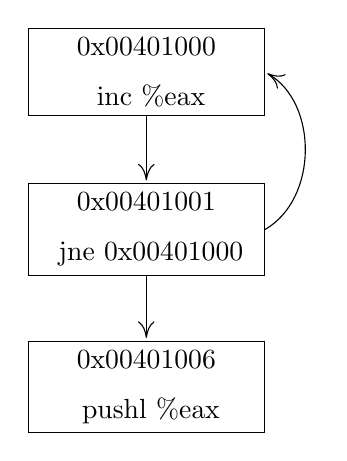
\begin{tikzpicture}[shorten >=1pt,node distance=2cm,on grid,auto] 
   	\node[cfgstate,align=center](s_1){0x00401000\\\ inc \%eax}; 
   	\node[cfgstate,align=center](s_2)[below of=s_1]{0x00401001\\\ jne 0x00401000};
   	\node[cfgstate,align=center](s_3)[below of=s_2]{0x00401006\\\ pushl \%eax};
    \path[-{>[scale=2,length=3,width=3]}] 
    (s_1) edge node {} (s_2)
  	(s_2.east) edge [bend right=60] node {} (s_1.east)
    (s_2) edge node {} (s_3);	  
\end{tikzpicture}
\caption{CFG của BE-PUM với đoạn mã assembly \ref {lst:IntroASM}}
\label{fig:IntroCFG}
\end{figure}

\hspace{0.5cm}Kế thừa bộ thư viện dịch ngược mã nhị phân của Jackstab, với mục tiêu có thể xây dựng hoàn chỉnh mô hình cho các tập tin thực thi, BE-PUM không chỉ dừng lại với việc phân tích tĩnh mà còn mở rộng để có thể phân tích động thông qua việc áp dụng các kỹ thuật bao gồm:

\begin{itemize}
\item{Dynamic symbolic execution: kỹ thuật nhằm tính toán các giá trị thanh ghi và bộ nhớ cụ thể từ đó có thể giải quyết vấn đề xử lý kỹ thuật trong đó sử dụng các câu lệnh nhảy động, nhảy có điều kiện - một kỹ thuật được sử dụng rất phổ biến trong hầu hết các malware và packer.\\}
\item{On-the-fly model generation: giải thuật chính được áp dụng trong hệ thống BE-PUM, do quá trình thực thi của tập tin mã nhị phân là thực thi động, do đó quá trình này sẽ bao gồm một dãy các câu lệnh mã nhị phân liên tiếp bắt đầu từ một giá trị trong bộ nhớ ở phân vùng mã, giá trị địa chỉ này được trỏ tới bởi giá trị thanh ghi EIP. Chính việc áp dụng giải thuật On-the-fly mà vấn đề thay đổi động giá trị opcode của các câu lệnh trong quá trình thực thi được giải quyết một cách triệt để, hay nói cách khác với những tập tin thực thi có sử dụng kỹ thuật self-modifcation code sẽ được BE-PUM hỗ trợ hoàn toàn.\\}
\item{Xử lý kỹ thuật obfuscation: điểm mạnh và là ưu thế vượt trội của BE-PUM so với các công cụ phân tích mã thực thi khác như Jackstab, IDA-Pro, Capstone, Unicorn, METASM, HOOPER đó là BE-PUM có hỗ trợ xử lý những kỹ thuật obfuscation như: indirect jump, self-modification code, entry point obscuring, strutured exception handling, overlapping instruction những kỹ thuật vốn được sử dụng rất phổ biến trong malware hay packer.}
\end{itemize}

\begin{code}
\begin{lstlisting}[captionpos=b,caption={Đoạn mã thực thi dưới dạng ASM},label={lst:ASMReal},frame=single]
start:
	cmp eax, 0
	jne A2
A1:
	add eax, 09h
	inc eax
	inc eax
	jmp eax
A2:
	mov eax, ss:[esp]
	ret
A3:
	push 0
	call ExitProcess
end start
\end{lstlisting}
\end{code} 

\begin{figure}
\centering
\begin{tabular}[c]{cc}
	\subfloat[BE-PUM]
	{
		\label{fig:BEPUMReal}
		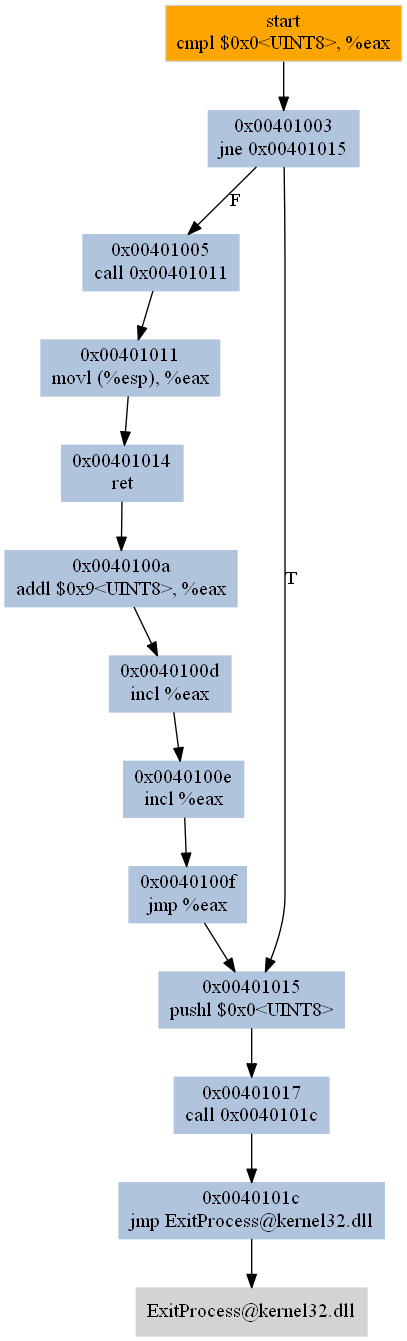
\includegraphics[width=0.4\textwidth]{bepum_sample}
    }
    &
	\subfloat[IDA-Pro]
	{
		\label{fig:IDAReal}
        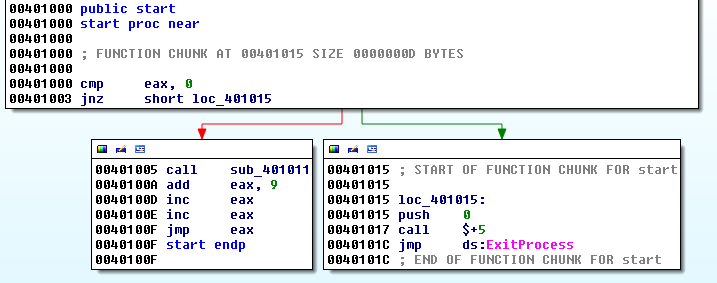
\includegraphics[width=0.6\textwidth]{ida_sample}
	}
\end{tabular}
\caption{Mô hình của BE-PUM và IDA Pro được sinh ra từ đoạn mã \ref {lst:ASMReal}}
\label{fig:ModelReal}
\end{figure}

\hspace{0.5cm}Hình \ref {fig:ModelReal} cho thấy công cụ IDA Pro, một công cụ rất mạnh được sử dụng cho quá trình phân tích tập tin mã nhị phân không thể xử lý kỹ thuật Indirect Jump tại câu lệnh JMP EAX tại vị trí 0x0040100f, cụ thể IDA Pro sẽ dừng thực thi và không nhảy đến được vị trí 0x00401015. Ngược lại hệ thống BE-PUM xử lý và nhảy đến vị trí 0x00401015 đã được tính toán trước đó.

\subsection{Tổng quan về Packer}

\begin{figure}
\centering
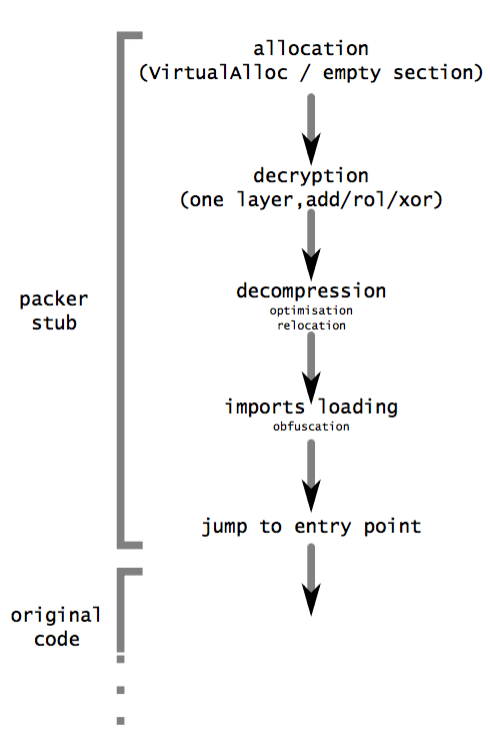
\includegraphics[width=0.5\textwidth]{simple_packer_schema}
\caption{Mô hình của một packer đơn giản}
\label{fig:PackerSchema}
\end{figure}

\hspace{0.5cm}Packer là những công cụ dùng để đóng gói một tập tin. Hình \ref {fig:PackerSchema} mô tả cấu trúc của một packer đơn giản. Trong đó có thể thấy mục tiêu chính của một packer có thể được chia làm 3 mục tiêu cụ thể là:

\begin{itemize}
\item{Giảm kích thước của tập tin: đây cũng là mục tiêu mà rất nhiều packer hướng tới, bằng việc áp dụng các kỹ thuật packing và self-unpacking, encryption và self-decryption, mà kích thước của một tập tin được đóng gói qua đó cũng giảm đi một cách đáng kể. Tuy nhiên, những packer hiện đại ngày nay đã không còn đặt tiêu chí giảm kích thước tập tin lên hàng đầu, bởi giảm kích thước đồng nghĩa với việc sử dụng những kỹ thuật bảo mật khác sẽ được loại bỏ và do đó độ tin cậy của một packer cũng giảm đi. Thậm chí những packer có cơ chế bảo mật tốt hiện nay có thể kể ra như Armadillo, Themida hay PEBundle có thể làm kích thước tập tin tăng lên rất nhiều lần do việc áp dụng kỹ thuật phức tạp của những packer này trên tập tin cần đóng gói là rất nhiều.\\}
\item{Chống dịch ngược: một trong những kỹ thuật được sử dụng rất nhiều trong việc tìm ra những lỗ hỏng của một phần mềm từ đó tìm cách đánh cắp dữ liệu mật của phần mềm đó hay tìm hiểu cơ chế sinh khoá, dịch ngược cũng được áp dụng để phát hiện những kỹ thuật malware từ đó tìm cách sửa lỗi hệ thống mà malware khai thác và chống lại malware đó. Nhằm chống lại kỹ thuật dịch ngược, packer cũng được sử dụng như một công cụ hiệu quả vì những giải thuật đóng gói tập tin phức tạp của packer có thể khiến việc dịch ngược mã nhị phân trở nên vô cùng khó khăn.\\}
\item{Bảo vệ bản quyền của phần mềm: đây cũng là mục tiêu chính yếu nhất mà các packer ngày nay hướng tới, bằng cách nâng cao độ phức tạp của các giải thuật đóng gói, đồng thời áp dụng những kỹ thuật anti-debugging, anti-reversing sẽ qua đó giúp bảo vệ một phần mềm khỏi việc đánh cắp thông tin bất hợp pháp. Malware cũng lợi dụng điểm mạnh này của packer nhằm che dấu quá trình thực thi của mình.}
\end{itemize}

\subsection{Tổng quan về Model Checking}

\hspace{0.5cm}Bài toán kiểm định các hệ thống phần mềm hay phần cứng là một bài toán vô cùng quan trọng và tốn rất nhiều thời gian và công sức nếu được thực hiện một cách thủ công, do đó việc đề ra một phương thức tự động nhằm kiểm định hệ thống là yêu cầu cần thiết được đề ra nhằm giải quyết vấn đề này. Chính vì điều này, mà việc xây dựng một phương pháp hình thức hay nói cách khác là việc áp dụng toán học để xử lý bài toán kiểm định sẽ mang lại hiệu quả và giảm rất nhiều thời gian, công sức.\\

\hspace{0.5cm}Model checking được xây dựng bởi Edmund Melson Clarke và Ernest Allen Emerson, cũng như Jean-Pierre Queille và Joseph Sifakis Jean-Pierre ra đời để giải quyết bài toán này. Model checking là một kỹ thuật kiểm định tự động một mô hình hệ thống với một đặc tả các tính năng của mô hình đó dưới dạng công thức logic có yếu tố thời gian. Bằng cách duyệt toàn bộ không gian trạng thái của mô hình đó, phương pháp model checking sẽ chứng minh mô hình có thoả mãn các tính chất đã được mô tả trước đó hay không.

\subsection{Tổng quan về NuSMV}

\hspace{0.5cm}NuSMV là một công cụ kiểm tra mô hình dạng ký hiệu mã nguồn mở, là một dự án kết hợp giữa ITC-IRST, viện nghiên cứu ở phía Đông Trento, Ý và đại học Carnegie Mellon. Chính vì mã nguồn mở mà thông qua đó có thể dễ dàng thay đổi mã nguồn để có thể cung cấp thêm nhiều tính năng và hỗ trợ tốt hơn, nâng cao hiệu suất kiểm tra mô hình trên hệ thống có số trạng thái hữu hạn.\\

\hspace{0.5cm}Giống như những công cụ kiểm tra mô hình khác, NuSMV cũng cần đầu vào là một mô hình cần được kiểm tra và một mô tả dưới dạng công thức luận lý có yếu tố thời gian để thực hiện việc kiểm tra mô hình. Mô hình NuSMV được biểu diễn dưới dạng ngôn ngữ SMV, NuSMV hỗ trợ cả CTL model checking và LTL model checking.

\section{Mục tiêu đề tài}

\hspace{0.5cm}Hệ thống BE-PUM được phát triển để có thể xây dựng được mô hình chính xác của chương trình thực thi, cụ thể là mô hình quá trình thực thi của malware, từ đó có thể nhận dạng được malware. Tuy nhiên, việc malware sử dụng packer để ẩn thân khiến quá trình xây dựng này trở nên khó khăn. Xuất phát từ khó khăn thực tế đó, mục tiêu của đề tài luận văn tốt nghiệp này hướng tới bao gồm:

\begin{itemize}
\item{Phân tích những kỹ thuật được sử dụng của các packer bao gồm nhóm kỹ thuật obfuscation, kỹ thuật anti-reversing, anti-debugging.\\} 
\item{Hỗ trợ hệ thống BE-PUM xử lý các kỹ thuật của packer để đảm bảo BE-PUM có thể phân tích hoàn toàn các packer, cụ thể, tìm ra được vị trí entry point thực sự của tập tin được đóng gói. Từ đó, có thể xây dựng chính xác mô hình quá trình thực thi của tập tin.\\}
\item{Nhận dạng packer thông qua chữ ký bằng phương pháp nhận dạng chữ ký được sử dụng trong thực tế.\\}
\item{Nhận dạng packer thông qua ngữ nghĩa bằng phương pháp model checking, cụ thể, kết hợp hệ thống BE-PUM và công cụ kiểm tra mô hình dạng ký hiệu NuSMV để kết luận một tập tin có đang được đóng gói bởi packer nào hay không.\\}
\item{So sánh độ hiệu quả giữa hai phương pháp nhận dạng packer, một là phương pháp nhận dạng chữ ký và hai là phương pháp nhận dạng ngữ nghĩa.}
\end{itemize}

\section{Phạm vi đề tài}

\hspace{0.5cm}Với những giới hạn trong việc chuyển đổi giữa mô hình của BE-PUM và mô hình của NuSMV, cũng như những khó khăn khi phân tích những packer hiện đại mà đề tài luận văn bao gồm những hạn chế cụ thể như sau:

\begin{itemize}
\item{Dữ liệu chữ ký của packer được sử dụng từ dữ liệu mở của phần mềm CFF Explorer, do đó BE-PUM chỉ hỗ trợ nhận dạng chữ ký những packer trong giới hạn cụ thể được định nghĩa tương tự như trong CFF Explorer.\\}
\item{Do sự phức tạp trong việc sử dụng kỹ thuật mới đòi hỏi xử lý Process, Thread phức tạp của các packer hiện đại như: Armadillo, Fastpack, Themida, PEBunble, mà những kỹ thuật này chưa được hỗ trợ hoàn toàn trong BE-PUM nên hiện tại BE-PUM chưa xử lý được những packer này, giới hạn đề tài chỉ hỗ trợ 27 packer.\\}
\item{Do BE-PUM chỉ xử lý được 27 packer và 14 kỹ thuật được sử dụng trong packer, nên giới hạn đề tài chỉ hỗ trợ nhận dạng 27 packer thông qua kiểm tra mô hình dựa trên mô tả của 14 kỹ thuật này.}
\end{itemize}  

\section{Kết quả đề tài}

\hspace{0.5cm}Nội dung và kết quả nghiên cứu được thực hiện trong đề tài luận văn này đã được vinh dự đóng góp trong bài báo "Precise Packer detection using Model checking" tại hội nghị SEATUC 2016 (10th SOUTH EAST ASIAN TECHNICAL UNIVERSITY CONSORTIUM SYMPOSIUM) được diễn ra tại Viện công nghệ Shibaura, Tokyo, Nhật Bản từ ngày 22/02/2016 đến ngày 24/02/2016.

\section{Cấu trúc của luận văn}

\hspace{0.5cm}Nội dung của luận văn tốt nghiệp bao gồm các chương chính như sau:

\begin{itemize}
\item{\textbf{Mở đầu}: giới thiệu sơ lược về đề tài luận văn, bố cục chung của luận văn, trình bày những mục tiêu khi chọn đề tài.\\}
\item{\textbf{Chương 1}: tập trung giới thiệu tổng quan về đề tài, cụ thể về hệ thống BE-PUM và cách thức xây dựng mô hình của BE-PUM, đồng thời giới thiệu về packer, phương pháp model checking và công cụ NuSMV; mục tiêu cụ thể hướng tới của đề tài và phạm vi thực hiện của đề tài, những kết quả ban đầu đã đạt được của quá trình nghiên cứu đề tài, cũng như cấu trúc của luận văn cũng sẽ được giới thiệu cụ thể.\\}
\item{\textbf{Chương 2}: tập trung phân tích vấn đề, cụ thể là những vấn đề của hệ thống BE-PUM khi xử lý packer thông qua 3 ví dụ cụ thể về 2 packer được malware sử dụng trong thực tế, rút ra nhận xét tổng quát và những thách thức đặt ra cho đề tài. Ngoài ra, chương này cũng sẽ tập trung bàn luận về những thách thức này, từ đó đưa ra những giải pháp cụ thể để giải quyết những khó khăn đó.\\}
\item{\textbf{Chương 3}: giới thiệu những kiến thức nền và các công nghệ được sử dụng trong đề tài. Để có thể giải quyết những thách thức như chương 2 đã nêu ra, cần nắm vững kiến thức nền tảng về hệ thống BE-PUM và lý thuyết về model checking, cũng như về công cụ NuSMV. Ngoài ra chương này cũng tập trung giới thiệu cụ thể về 14 kỹ thuật được hỗ trợ trong packer.\\}
\item{\textbf{Chương 4}: trình bày về các công việc đã thực hiện trong luận văn dựa trên những kiến thức nền được giới thiệu ở chương 2. Cụ thể, chương này sẽ tập trung giới thiệu việc kết hợp giữa hệ thống BE-PUM và công cụ NuSMV trong việc nhận dạng packer. Để có thể so sánh giữa phương pháp pháp nhận dạng packer thông qua chữ ký và phương pháp model checking, giải thuật nhận dạng packer thông qua chữ ký cũng được hiện thực và giới thiệu cụ thể trong chương này.\\}
\item{\textbf{Chương 5}: chủ yếu trình bày những kết quả đã đạt được sau khi thực hiện đề tài, kết quả thí nghiệm trên tập malware thực tế, cũng như những so sánh giữa 2 phương pháp nhận dạng packer.\\}
\item{\textbf{Chương 6}: nêu ra những hạn chế được đặt ra trong quá trình thực hiện đề tài và hướng giải quyết trong tương lai để có thể khắc phục những hạn chế đó.}
\end{itemize}



% ==========================================
% PROBLEMS AND CHALLENGES
% ==========================================

\newpage
\chapter{PHÂN TÍCH VẤN ĐỀ}

\begin{concept}[15cm]
\textit{Nội dung chương này sẽ tập trung phân tích vấn đề được đặt ra trong đề tài, cụ thể là những vấn đề của hệ thống BE-PUM khi xử lý packer thông qua 3 ví dụ cụ thể về 2 packer được malware sử dụng trong thực tế, rút ra nhận xét tổng quát và những thách thức đặt ra cho đề tài. Ngoài ra, chương này cũng sẽ tập trung bàn luận về những thách thức này, từ đó đưa ra những giải pháp cụ thể để giải quyết những khó khăn đó.}
\end{concept}

\section{Ví dụ thực tế}\label{sec:Example}

\subsection{Ví dụ 1}\label{subsec:Example1}

\hspace{0.5cm}Không chỉ thay đổi giải thuật phức tạp nhằm đóng gói mã thực thi, packer còn sử dụng các kỹ thuật obfuscation ngày càng tinh vi hơn. Ví dụ \ref {subsec:Example1} sẽ trình bày cụ thể về packer TELOCK được malware sử dụng trong thực tế sử dụng kỹ thuật Strutured Exception Handler dựa trên Trap Flag:

\begin{code}
\begin{lstlisting}[captionpos=b,caption={Kỹ thuật Structured Exception Handler sử dụng trong packer TELOCK},label={lst:ASMExample1},frame=single]
00405A27	call 0x00405A32
00405A2C	mov esp, ss:[esp]
00405A30	jmp 0x00405A4C
00405A32	push fs:[0]
00405A38	mov fs:[0], esp
00405A3E	pushfd
00405A3F	or ss:[esp], 0x100
00405A46	popfd
00405A47	clc
00405A48	jnb 0x00405A32
\end{lstlisting}
\end{code}

\begin{figure}
\centering
\begin{tabular}[c]{cc}
	\subfloat[Trước]
	{
		\label{fig:BeforeExample1}
		\resizebox{6cm}{!}{
		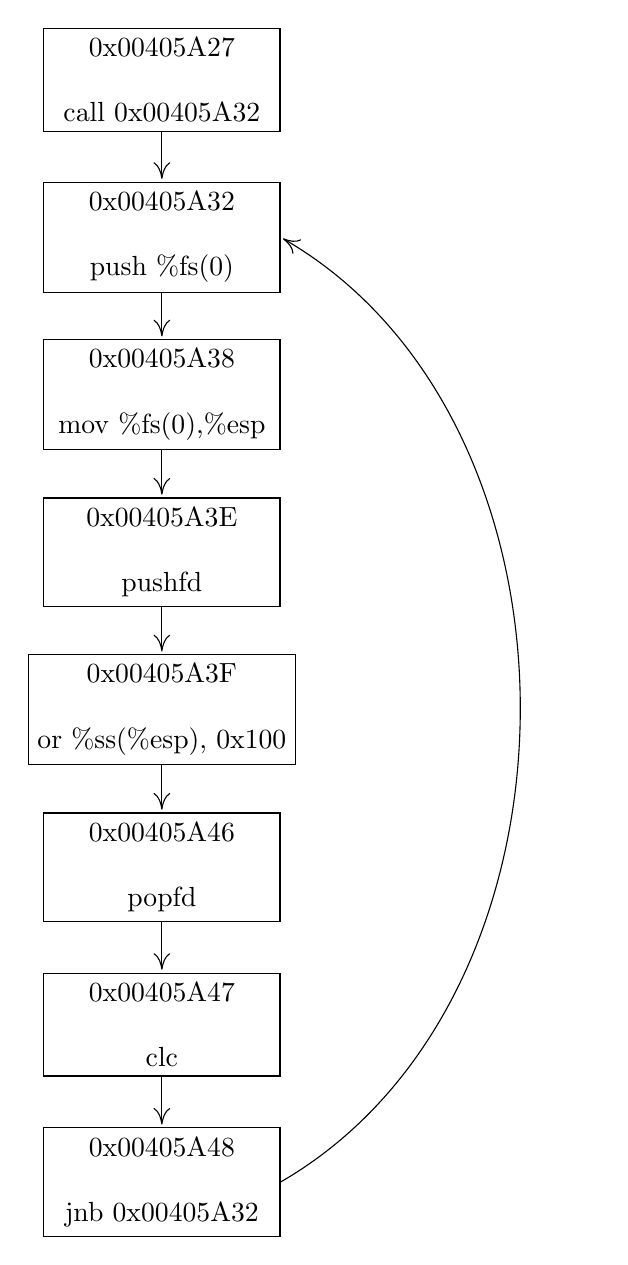
\begin{tikzpicture}[shorten >=1pt,node distance=2cm,on grid,auto] 
		   	\node[cfgstate,align=center](s_1){0x00405A27\\[0.2cm] call 0x00405A32}; 
		   	\node[cfgstate,align=center](s_2)[below of=s_1]{0x00405A32\\[0.2cm] push \%fs(0)};
		   	\node[cfgstate,align=center](s_3)[below of=s_2]{0x00405A38\\[0.2cm] mov \%fs(0),\%esp};
		   	\node[cfgstate,align=center](s_4)[below of=s_3]{0x00405A3E\\[0.2cm] pushfd};
		   	\node[cfgstate,align=center](s_5)[below of=s_4]{0x00405A3F\\[0.2cm] or \%ss(\%esp), 0x100};
		   	\node[cfgstate,align=center](s_6)[below of=s_5]{0x00405A46\\[0.2cm] popfd};
		   	\node[cfgstate,align=center](s_7)[below of=s_6]{0x00405A47\\[0.2cm] clc};
		   	\node[cfgstate,align=center](s_8)[below of=s_7]{0x00405A48\\[0.2cm] jnb 0x00405A32};
		    \path[-{>[scale=2,length=3,width=3]}] 
		    (s_1) edge node {} (s_2)
		    (s_2) edge node {} (s_3)
		   	(s_3) edge node {} (s_4)
		   	(s_4) edge node {} (s_5)
		   	(s_5) edge node {} (s_6)
		   	(s_6) edge node {} (s_7)
		   	(s_7) edge node {} (s_8)
		   	(s_8.east) edge [bend right=60] node {} (s_2.east);
		\end{tikzpicture}
		}
    }
    &
	\subfloat[Sau]
	{
		\label{fig:AfterExample1}
		\resizebox{4cm}{!}{
        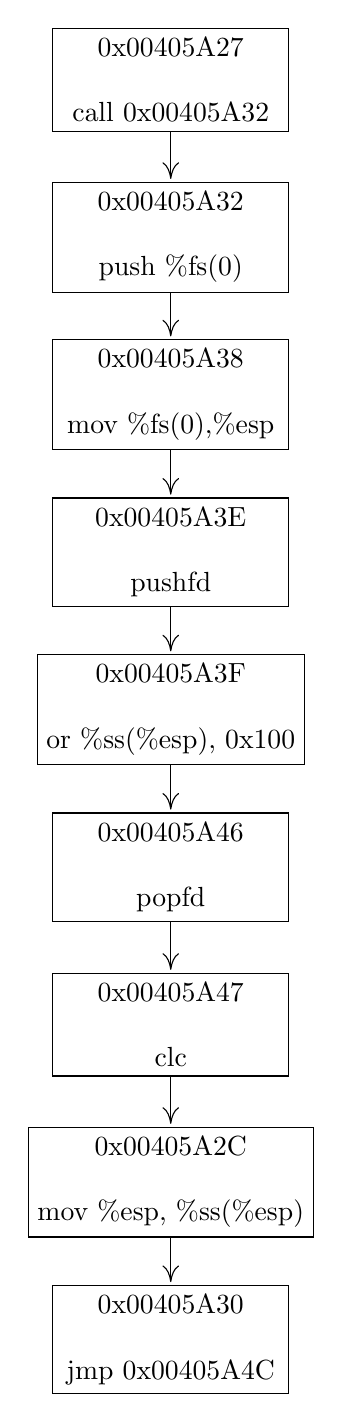
\begin{tikzpicture}[shorten >=1pt,node distance=2cm,on grid,auto] 
		   	\node[cfgstate,align=center](s_1){0x00405A27\\[0.2cm] call 0x00405A32}; 
		   	\node[cfgstate,align=center](s_2)[below of=s_1]{0x00405A32\\[0.2cm] push \%fs(0)};
		   	\node[cfgstate,align=center](s_3)[below of=s_2]{0x00405A38\\[0.2cm] mov \%fs(0),\%esp};
		   	\node[cfgstate,align=center](s_4)[below of=s_3]{0x00405A3E\\[0.2cm] pushfd};
		   	\node[cfgstate,align=center](s_5)[below of=s_4]{0x00405A3F\\[0.2cm] or \%ss(\%esp), 0x100};
		   	\node[cfgstate,align=center](s_6)[below of=s_5]{0x00405A46\\[0.2cm] popfd};
		   	\node[cfgstate,align=center](s_7)[below of=s_6]{0x00405A47\\[0.2cm] clc};
		   	\node[cfgstate,align=center](s_8)[below of=s_7]{0x00405A2C\\[0.2cm] mov \%esp, \%ss(\%esp)};
		   	\node[cfgstate,align=center](s_9)[below of=s_8]{0x00405A30\\[0.2cm] jmp 0x00405A4C};
		    \path[-{>[scale=2,length=3,width=3]}] 
		    (s_1) edge node {} (s_2)
		    (s_2) edge node {} (s_3)
		   	(s_3) edge node {} (s_4)
		   	(s_4) edge node {} (s_5)
		   	(s_5) edge node {} (s_6)
		   	(s_6) edge node {} (s_7)
		   	(s_7) edge node {} (s_8)
		   	(s_8) edge node {} (s_9);
		\end{tikzpicture}
		}
	}
\end{tabular}
\caption{CFG của BE-PUM trước và sau khi xử lý packer TELOCK}
\label{fig:CFGExample1}
\end{figure}

\hspace{0.5cm}Trong mô hình \ref {fig:CFGExample1} được sinh ra từ đoạn mã \ref {lst:ASMExample1} có thể thấy giá trị của thanh ghi cờ EFLAGS sẽ bị thay đổi qua câu lệnh tại địa chỉ 0x00405A3F, qua đó sẽ thay đổi giá trị của Trap Flag thành TRUE, chính vì giá trị này thay đổi sẽ gây ra một exception trong chương trình với kiểu SINGLE\_STEP\_EXCEPTION. Khi đó luồng thực thi sẽ thay đổi và trỏ tới hàm xử lý exception với điểm nhập là giá trị địa chỉ được lưu trong bộ nhớ tại vị trí FS:[0]. Hệ thống BE-PUM chưa hỗ trợ Trap Flag do đó sẽ dẫn tới vòng lặp vô tận tại vị trí 0x00405A32, khi đó stack sẽ được push liên tục và dẫn đến chương trình gọi ExitProcess để giải phóng bộ nhớ.

\subsection{Ví dụ 2}\label{subsec:Example2}

\hspace{0.5cm}Trong thực tế, một malware để tránh bị phát hiện bởi một chương trình chống malware, có thể sử dụng packer để ẩn thân hay nói cách khác che dấu điểm nhập thực sự của mình. Cụ thể malware sẽ sử dụng packer để đóng gói đoạn code thực thi thực sự của mình, và tự mở gói bằng kỹ thuật self-unpacking. Ví dụ \ref {subsec:Example2} sẽ trình bày cụ thể về packer FSG được malware sử dụng trong thực tế có sử dụng kỹ thuật packing và self-unpacking:

\begin{code}
\begin{lstlisting}[captionpos=b,caption={Kỹ thuật Unpacking sử dụng trong packer FSG},label={lst:ASMExample2},frame=single]
004001A1	cmp eax, ds:[ebx-8]
004001A4	jnb 0x004001B0
...
004001B0	inc ecx
004001B1	inc ecx
004001B2	xchg eax, ebp
004001B3	mov eax, ebp
004001B5	mov dh, 0
004001B7	push esi
004001B8	mov esi, edi
004001BA	sub esi, eax
004001BC	rep movs es:[edi], ds:[esi]
004001BE	pop esi
004001BF 	jmp 0x00400160		
...
004001D1	jmp ds:[ebx+C]
\end{lstlisting}
\end{code} 

\hspace{0.5cm}Trong đoạn mã \ref {lst:ASMExample2} có thể thấy quá trình mở gói được thực hiện thông qua việc sử dụng các câu lệnh tính toán và kết thúc là một lệnh nhảy tại địa chỉ 0x004001D1 tới vị trí 0x00401000 trong bộ nhớ, mà vị trí này là vị trí entry point thực sự của tập tin trước khi đóng gói. Vị trí này cũng chính là vị trí mà quá trình mở gói sẽ thay đổi giá trị mã liên tục cho tới khi quá trình kết thúc. 

\subsection{Ví dụ 3}\label{subsec:Example3}

\hspace{0.5cm}Đối với những packer hiện đại ngày nay, không chỉ nâng cấp độ phức tạp của giải thuật đóng gói bằng việc sử dụng rất nhiều câu lệnh tính toán phức tạp, những packer này còn áp dụng rất nhiều kỹ thuật anti-reversing, anti-debugging nhằm khiến cho quá trình dịch ngược hay gỡ lỗi trở nên khó khăn rất nhiều. Ví dụ \ref {subsec:Example3} sẽ trình bày cụ thể về packer TELOCK được malware sử dụng trong thực tế có sử dụng kỹ thuật Hardware Breakpoint nhằm che dấu quá trình mở gói:

\begin{code}
\begin{lstlisting}[captionpos=b,caption={Kỹ thuật Hardware Breakpoints sử dụng trong packer TELOCK},label={lst:ASMExample3},frame=single]
00404083	push 0x004040C5
00404084	xor eax, eax
00404086	push fs:[eax]
00404089	mov fs:[eax],esp
0040408C 	int3
0040408D 	nop
0040408E 	mov eax, eax 
00404090 	stc
...
00404099 	clc
...
0040409E 	cld
...
004040A3 	nop
\end{lstlisting}
\end{code}

\hspace{0.5cm}Trong đoạn mã \ref {lst:ASMExample3} có thể thấy TELOCK packer sẽ gây ra một exception trong chương trình bằng việc sử dụng câu lệnh INT3, sau khi ngắt chương trình, luồng thực thi sẽ được thay đổi tới vị trí của hàm xử lý exception. Tại đây, các giá trị của các thanh ghi debug sẽ được thay đổi đến các giá trị 0x00404090, 0x00404099, 0x0040409E, 0x004040A3 tương ứng, chính vì các thanh ghi debug được kích hoạt sẽ dẫn đến exception xảy ra liên tục trong chương trình tại các vị trí trên. Nếu chương trình đang được phân tích trong môi trường debugger thì các exception này sẽ được bỏ qua dẫn đến quá trình mở gói sau sẽ không được thực thi chính xác.   

\subsection{Nhận xét vấn đề}

\hspace{0.5cm}Những ví dụ được đưa ra ở trên là những kỹ thuật nổi bật thuộc 2 nhóm kỹ thuật gồm: nhóm kỹ thuật obfuscation và nhóm kỹ thuật anti-reversing mà những kỹ thuật này được sử dụng rất phổ biến và là đặc trưng trong hầu hết các packer, những kỹ thuật này sẽ cản trở quá trình phân tích dịch ngược, gỡ lỗi nhằm che dấu điểm nhập chính thực sự của chương trình. Đối với những chương trình chỉ hỗ trợ quá tình phân tích tĩnh tập tin thực thi như: Jackstab, Capstone, Unicorn hay IDAPro vốn không xử lý được kỹ thuật self-modification code, là kỹ thuật lõi trong kỹ thuật unpacking của packer, hay không hỗ trợ việc xử lý, truy cập vào vùng memory nói chung và stack nói riêng, sẽ không thể hoặc hoàn toàn không có khả năng để xử lý các kỹ thuật trên. Do đó việc sử dụng một chương trình cho phép phân tích động, cụ thể là hệ thống BE-PUM là cần thiết và là giải pháp chung để phân tích một packer.

\section{Phân tích}

\subsection {Phân tích Packer trên hệ thống BE-PUM}

\hspace{0.5cm}Việc phân tích hoàn toàn một packer và tìm ra điểm nhập thực sự của chương trình là một vấn đề vô cùng quan trọng bởi từ đó mới có thể xây dựng hoàn chỉnh được quá trình thực thi của một malware và từ đó quá trình nhận dạng malware đó mới thực sự khả thi. Phân tích vấn đề được đưa ra trong 3 ví dụ trong chương \ref {sec:example} sẽ giúp cụ thể hoá những thách thức gặp phải của hệ thống BE-PUM trong quá trình phân tích packer, từ đó sẽ tìm ra được các công việc cần phải thực hiện trong quá trình xử lý này.\\

\hspace{0.5cm}Hệ thống BE-PUM hỗ trợ phân tích động một tập tin mã nhị phân, quá trình phân tích một packer đặt ra các yêu cầu đối với hệ thống BE-PUM như sau:

\begin{itemize}
\item{Packer sử dụng các kỹ thuật thuộc nhóm kỹ thuật obfuscation, cụ thể được nêu ra ở ví dụ 1 và ví dụ 2 chương \ref {sec:Example}. Đối với các chương trình phân tích tĩnh, quá trình thay đổi luồng thực thi, cũng như tự thay đổi mã sẽ khiến cho việc xử lý là bất khả thi. Hệ thống BE-PUM đã xử lý được những kỹ thuật obfuscation tuy nhiên với một biến thể mới như trong ví dụ đã nêu, BE-PUM sẽ gặp rất nhiều khó khăn. Từ đó cho thấy công việc cần thực hiện là hỗ trợ cho hệ thống BE-PUM để xử lý tốt hơn và hiệu quả hơn các kỹ thuật này.\\}
\item{Packer sử dụng rất nhiều kỹ thuật đa dạng nhằm phát hiện nếu chương trình thực thi đang được phân tích trong môi trường debugger bằng cách sử dụng các kỹ thuật thuộc nhóm kỹ thuật anti-reversing, anti-debugging như được nêu ra trong ví dụ 3 chương \ref {sec:Example}. Do đó, công việc cần thực hiện là hỗ trợ BE-PUM xử lý các kỹ thuật này, cụ thể hơn, cần phải giả lập một môi trường thực thi thực sự cho tập tin được đóng gói.}
\end{itemize}

\subsection {Nhận dạng Packer}

\hspace{0.5cm}Sau khi phân tích được một packer hoàn toàn trên hệ thống BE-PUM, đồng nghĩa với việc xây dựng được mô hình cho quá trình thực thi của một packer. Vậy làm cách nào để có thể nhận dạng được một tập tin có được đóng gói bởi một packer nào hay không khi chỉ có mô hình của quá trình thực thi tập tin bất kì. Do đó những yêu cầu mới được đặt ra như sau:

\begin{itemize}
\item{Xây dựng giải thuật nhận dạng packer thông qua chữ ký dựa trên dữ liệu chữ ký được thu thập. Tích hợp nhận dạng packer bằng chữ ký như một phần của hệ thống BE-PUM.\\}
\item{Với những malware, việc thay đổi chữ ký là một vấn đề gây khó khăn cho giải pháp nhận dạng chữ ký, đòi hỏi cơ sở dữ liệu lớn và cập nhật thường xuyên vì chỉ cần sự thay đổi duy nhất một byte trong chữ ký cũng sẽ sinh ra một chữ ký mới. Do đó yêu cầu mới đặt ra là xây dựng giải thuật nhận dạng packer thông qua ngữ nghĩa dựa trên phương pháp model checking, cụ thể kết hợp giữa hệ thống BE-PUM và công cụ NuSMV. Do đó, yêu cầu đặt ra là chuyển đổi từ mô hình được sinh ra bởi hệ thống BE-PUM sang mô hình NuSMV như đầu vào của công cụ NuSMV. Tích hợp nhận dạng packer thông qua công cụ NuSMV như một phần của hệ thống BE-PUM.}
\end{itemize}

\section{Giải pháp đề nghị}

\subsection {Thu thập và xử lý các kỹ thuật Packer}

\hspace{0.5cm}Để có thể đáp ứng được những yêu cầu được đặt ra trong quá trình xử lý và phân tích hoàn toàn một packer, giải pháp được đưa ra bao gồm:

\begin{itemize}
\item{Phân tích luồng thực thi của packer đó bằng một công cụ emulator hỗ trợ giả lập môi trường debugger như OllyDBG, cho phép phân tích từng câu lệnh thực thi, từ đó tìm ra những kỹ thuật mới của packer.\\}
\item{Tiến hành phân tích kỹ thuật đó trên hệ thống BE-PUM, hỗ trợ hệ thống BE-PUM xử lý kỹ thuật nếu quá trình phân tích gặp lỗi, quá trình phân tích là thành công khi tìm ra được điểm nhập thực sự của một chương trình. Khi đó có thể kết luận tập tin đã được mở gói thành công.\\}
\item{Thu thập các kỹ thuật đã được phân tích của các packer và xây dựng mẫu hành vi cho các kỹ thuật này.}
\end{itemize} 

\subsection {Nhận dạng Packer thông qua chữ ký}

\hspace{0.5cm}Nhận dạng thông qua chữ ký được sử dụng chủ yếu trong các phần mềm nổi tiếng như: PEID và CFF Explorer, những hạn chế về dữ liệu chữ ký là vấn đề không tránh khỏi khi nhận dạng packer theo phương pháp này. Để có thể đưa ra một sự so sánh về hiệu quả giữa 2 phương pháp nhận dạng packer được chọn, quá trình xây dựng giải thuật nhận dạng packer thông qua chữ ký được tích hợp trong hệ thống BE-PUM sẽ bao gồm:

\begin{itemize}
\item{Thu thập dữ liệu chữ ký của các packer.\\}
\item{Chuyển đổi dữ liệu chữ ký thô và lưu trữ dữ liệu này dưới dạng dữ liệu JSON.\\}
\item{Xây dựng giải thuật để nhận dạng chữ ký này trên packer.}
\end{itemize} 

\subsection {Nhận dạng Packer thông qua ngữ nghĩa}

\begin{figure}
\centering
\begin{tikzpicture}[node distance=1.5cm]
\node (s1) [statement] {Hành vi của packer};
\node (s2) [statement, right=4cm of s1] {Tập tin thực thi};
\node (p1) [process, below of=s1] {Hình thức hoá};
\node (p2) [process, below of=s2] {Mô hình hoá bằng hệ thống BE-PUM};
\node (s3) [statement, below of=p1] {Biểu thức CTL/LTL};
\node (s4) [statement, below of=p2] {CFG};
\node (s7) [statement, below of=s4] {Mô hình NuSMV};
\node (p3) [process, below = of $(s3)!0.5!(s7)$] {Công cụ NuSMV};
\node (d1) [decision, below=1cm of p3, align=center] {Thoả mãn \\\ tính chất ?};
\node (s5) [statement, below=1cm of d1] {Packer};
\node (s6) [statement, right=1cm of d1] {Chưa xác định};
\draw [arrow] (s1) -- (p1);
\draw [arrow] (s2) -- (p2);
\draw [arrow] (p1) -- (s3);
\draw [arrow] (p2) -- (s4);
\draw [arrow] (s3) |- (p3);
\draw [arrow] (s4) -- (s7);
\draw [arrow] (s7) |- (p3);
\draw [arrow] (p3) -- (d1);
\draw [arrow] (d1) -- node[anchor=east]{TRUE}(s5);
\draw [arrow] (d1) -- node[anchor=south]{FALSE}(s6);
\end{tikzpicture}
\caption{Kết hợp mô hình của BE-PUM và công cụ NuSMV} 
\label{fig:BepumwithNusmv}
\end{figure}

\hspace{0.5cm}Chính vì những hạn chế dễ nhận thấy của phương pháp chữ ký. Hình \ref {fig:BepumwithNusmv} mô tả quá trình kết hợp giữa hệ thống BE-PUM và công cụ NuSMV để có thể nhận dạng packe. Qua đó có thể thấy xây dựng giải thuật nhận dạng packer thông qua ngữ nghĩa hay sử dụng phương pháp model checking sẽ bao gồm:

\begin{itemize}
\item{Chuyển đổi mô hình được sinh ra bởi BE-PUM sang mô hình NuSMV.\\}
\item{Mô tả các mẫu hành vi của packer dưới dạng công thức CTL, LTL.\\}
\item{Sử dụng công cụ kiểm tra mô hình NuSMV với đầu vào là mô hình NuSMV đã được chuyển đổi và hành vi của packer, để kiểm tra tập tin có đang được đóng gói hay không.}
\end{itemize} 



% ==========================================
% BASE KNOWLEDGES
% ==========================================

\newpage
\chapter{KIẾN THỨC NỀN}

\begin{concept}[15cm]
\textit{Nội dung chương này sẽ giới thiệu những kiến thức nền và các công nghệ được sử dụng trong đề tài. Để có thể giải quyết những thách thức như chương 2 đã nêu ra, cần nắm vững kiến thức nền tảng về hệ thống BE-PUM và lý thuyết về model checking, cũng như về công cụ NuSMV. Ngoài ra chương này cũng tập trung giới thiệu cụ thể về 14 kỹ thuật được hỗ trợ trong packer.}
\end{concept}

\section{Hệ thống BE-PUM}

\subsection{Kiến trúc của BE-PUM}

\hspace{0.5cm}Hệ thống BE-PUM xây dựng mô hình quá trình thực thi của một tập tin thực thi dựa trên kỹ thuật Dynamic symbolic execution. BE-PUM dựa trên thư viện mã nguồn mở Jackstab để dịch ngược mã nhị phân cho từng câu lệnh hợp ngữ tương ứng với từng câu lệnh thực thi của tập tin và chương trình Z3 để tìm ra đường đi nếu câu lệnh thực thi là một câu lệnh nhảy hoặc nhảy có điều kiện.

\begin{figure}[h]
\centering
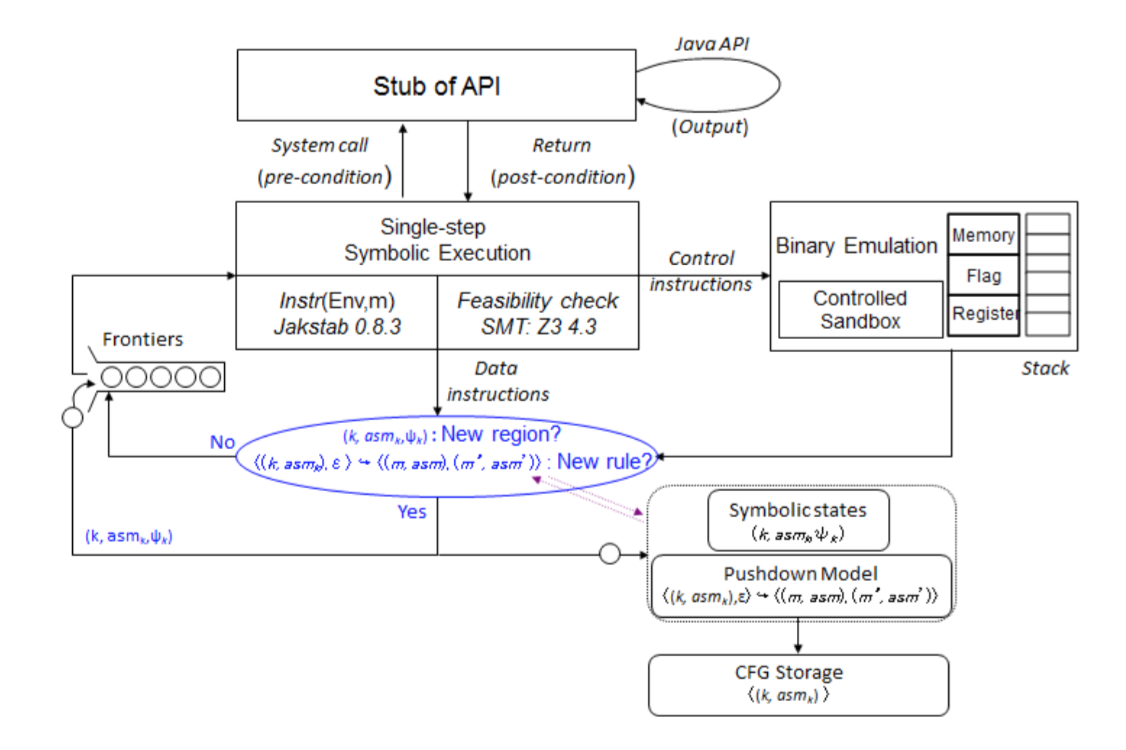
\includegraphics[width=0.7\textwidth]{bepum_architecture}
\caption{Kiến trúc của hệ thống BE-PUM}
\label{fig:BepumArchi}
\end{figure}

\hspace{0.5cm}Kiến trúc của hệ thống BE-PUM bao gồm 3 thành phần chính: symbolic execution, binary emulation và CFG storage. Hình \ref {fig:BepumArchi} mô tả kiến trúc của hệ thống BE-PUM. Trong đó, vai trò của các thành phần này như sau:

\begin{itemize}
\item{Single-step symbolic execution: sử dụng Jackstab để dịch ngược và chuyển đổi thành câu lệnh hợp ngữ tương ứng. Nếu câu lệnh hợp ngữ là câu lệnh chỉ tác động tới môi trường thực thi, cụ thể là các câu lệnh tính toán, câu lệnh ghi hoặc đọc trong bộ nhớ, bao gồm cả stack. Khi đó chỉ có môi trường thực thi được thay đổi và vị trí của câu lệnh tiếp theo chỉ được xác định bằng vị trí của câu lệnh hiện tại và kích thước câu lệnh. Nếu câu lệnh tiếp theo là câu lệnh điều khiển, cụ thể là các câu lệnh gọi hàm, câu lệnh trả về từ hàm, câu lệnh nhảy và câu lệnh nhảy có điều kiện, thì câu lệnh tiếp theo sẽ được tính toán thông qua dynamic symbolic execution.\\}
\item{
\begin{figure}[h]
\centering
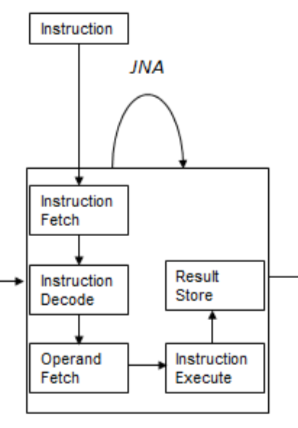
\includegraphics[width=0.3\textwidth]{bepum_binary_emulation}
\caption{Thành phần Binary Emulation trong BE-PUM}
\label{fig:BepumBE}
\end{figure}
Binary emulation: là thành phần quan trọng trong tổng thể kiến trúc của BE-PUM. Để có thể xử lý một câu lệnh hợp ngữ, hệ thống BE-PUM sẽ giả lập các thành phần của hệ thống, cụ thể là mô hình bộ nhớ của BE-PUM, mô hình này bao gồm tập 9 cờ được sử dụng trong hệ thống (AF, CF, DF, IF, OF, PF, SF, TF, và ZF), tập 20 thanh ghi (EAX, EBX, ECX, EDX, ESI, EDI, ESP, EBP, CS, DS, ES, FS, GS, SS, EIP, EFLAGS và 8 thanh ghi debug DRO, DR1, DR2, DR3, DR4, DR5, DR6, DR7, DR8), tập các giá trị bộ nhớ được lưu trữ trong đó một phần của bộ nhớ cho stack được giới hạn bởi thanh ghi esp và thanh ghi ebp. Bộ nhớ được giả lập trong BE-PUM được lưu trữ dưới dạng từng byte một. Ngoài việc giả lập câu lệnh hợp ngữ, thì API cũng được giả lập thông qua sử dụng Java Native Access cho phép gọi trực tiếp từ các thư viện liên kết động, trong đó giá trị trả về của các API sẽ được lưu trữ trong các thanh ghi tương ứng. Đối với các API đặc biệt tác động trực tiếp đến môi trường thực, một sandbox sẽ được xây dựng cho quá trình xử lý các API này. Ngoài ra, các API được sử dụng như một phần của kỹ thuật anti-reversing, anti-debugging, giá trị trả về sẽ là một giá trị symbolic. Hình \ref {fig:BepumBE} mô tả các quá trình xử lý một câu lệnh thực thi trong hệ thống BE-PUM.\\
}
\item{CFG storage: được sử dụng để lưu trữ một CFG node và CFG edge sau khi được tính toán chính xác. CFG storage sẽ được sử dụng để xây dựng mô hình quá trình thực thi cuối cùng của tập tin được phân tích.}
\end{itemize}

\subsection{Mô hình của BE-PUM}
\hspace{0.5cm}Kết quả của quá trình phân tích một tập tin thực thi là một mô hình quá trình thực thi, mô hình được sinh ra bởi hệ thống BE-PUM được biểu diễn dưới dạng Control Flow Graph hay CFG của chương trình.\\

\hspace{0.5cm}Một CFG là một tập của các node và edge. Trong đó một node của CFG bao gồm địa chỉ của câu lệnh và câu lệnh hợp ngữ tại địa chỉ đó, một edge của CFG là cạnh nối giữa 2 node của CFG.

\begin{code}
\begin{lstlisting}[captionpos=b,caption={Ví dụ về một đoạn mã thực thi},label={lst:SampleExeASM},frame=single]
00401000  pushl 0x00401007
00401005  xor eax, eax
00401007  jne 0x00401005
0040100B  call ss:[esp]		
\end{lstlisting}
\end{code}

\hspace{0.5cm}Với đoạn mã \ref {lst:SampleExeASM}, quá trình phân tích trên hệ thống BE-PUM sẽ sinh ra được mô hình của đoạn mã thực thi hay CFG của chương trình thực thi trên như sau:

\begin{figure}
\centering
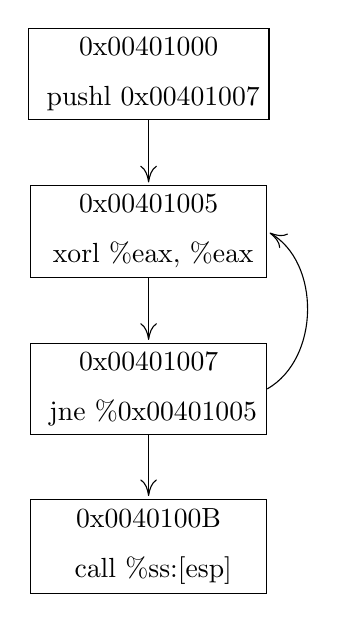
\begin{tikzpicture}[shorten >=1pt,node distance=2cm,on grid,auto] 
   	\node[cfgstate,align=center](s_1){0x00401000\\\ pushl 0x00401007}; 
   	\node[cfgstate,align=center](s_2)[below of=s_1]{0x00401005\\\ xorl \%eax, \%eax};
    \node[cfgstate,align=center](s_3)[below of=s_2]{0x00401007\\\ jne \%0x00401005};
   	\node[cfgstate,align=center](s_4)[below of=s_3]{0x0040100B\\\ call \%ss:[esp]};
    \path[-{>[scale=2,length=3,width=3]}] 
    (s_1) edge node {} (s_2)
    (s_2) edge node {} (s_3)
  	(s_3.east) edge [bend right=60] node {} (s_2.east)
    (s_3) edge node {} (s_4);	  
\end{tikzpicture}
\label{fig:SampleExeCFG}
\caption{CFG được sinh ra từ đoạn mã thực thi \ref {lst:SampleExeASM}}
\end{figure}

\subsection{Hạn chế của BE-PUM}

\hspace{0.5cm}Một số những hạn chế của hệ thống BE-PUM bao gồm:

\begin{itemize}
\item{Số lượng các câu lệnh hợp ngữ là rất lớn khoảng hơn 1000 câu lệnh và số lượng API là 4000. Tuy nhiên hiện tại BE-PUM chỉ hõ trợ được 200 câu lệnh và 400 API. Do đó đối với các malware hay packer sử dụng những câu lệnh hay API không được hỗ trợ, BE-PUM sẽ không thể phân tích tiếp tục được và do đó quá trình phân tích sẽ kết thúc.\\}
\item{Đối với những malware hay packer sử dụng những vòng lặp lớn hơn 1 tỷ lần thì quá trình phân tích trên BE-PUM sẽ kết thúc. Do đó khi gặp một vòng lặp với số lượng lớn thì quá trình phân tích sẽ tiếp tục được phân tích trên một đường thực thi khác.\\}
\item{Trong thực tế, trước khi thực thi tại entry point của chương trình, một số xử lý từ hệ điều hành sẽ được thực hiện qua đó tác động đến các giá trị thanh ghi, bộ nhớ và stack tại entry point. Do đó, khi quá trình phân tích bắt đầu, tại vị trí entry point, hệ thống BE-PUM sẽ mặc định thiết lập các giá trị mặc định cho stack bao gồm: địa chỉ chứa mã ASCII của tên tập tin, địa chỉ hàm xử lý exception của hệ thống, và giá trị trả về là một giá trị bất kì thuộc địa chỉ kernel.\\}
\item{Ngoài ra, các giá trị cờ cũng được thiết lập cụ thể như mô tả trong bảng \ref {table:BepumInitFlag}. Đối với các thanh ghi EAX, CS, DS, ES, FS, GS, SS, EFLAGS được thiết lập giá trị symbolic, các thanh ghi được thiết lập như mô tả trong bảng \ref {table:BepumInitReg}.
}
\end{itemize}

\begin{longtable}{ | m{2cm} | m{5cm} | }
\hline 
CF & False\\
\hline 
PF & True\\
\hline 
AF & False\\
\hline 
ZF & True\\
\hline 
SF & False\\
\hline 
TF & False\\
\hline 
DF & False\\
\hline 
OF & False\\
\hline 
IF & False\\
\hline
\caption{Các giá trị cờ được khởi tạo mặc định trong hệ thống BE-PUM}
\label{table:BepumInitFlag}
\end{longtable}

\begin{longtable}{ | m{5cm} | m{5cm} | }
\hline 
EIP, EDX & Địa chỉ entry point\\
\hline
ESP & Địa chỉ đỉnh của stack\\
\hline
EBP & Địa chỉ cơ sở của stack\\
\hline
ECX, EDI, ESI & 0\\
\hline
EBX & Địa chỉ PEB\\
\hline
\caption{Các giá trị thanh ghi được khởi tạo mặc định trong hệ thống BE-PUM}
\label{table:BepumInitReg}
\end{longtable}

\section{Model Checking và NuSMV}

\subsection{Model Checking}

\hspace{0.5cm}Model checking hay kiểm tra mô hình là một kỹ thuật tự động được sử dụng để kiểm tra một hệ thống tuần tự có số trạng thái hữu hạn bằng việc vét cạn toàn bộ không gian trạng thái của mô hình hệ thống. Bằng việc cung cấp một mô hình của hệ thống và một mô tả hành vi hệ thống cần kiểm tra dưới dạng biểu thức logic có yếu tố thời gian, phương pháp model checking có thể kết luận mô hình được kiểm tra có thoả mãn các tính chất được mô tả hay không. Hay nói một cách khác, với một mô hình hệ thống với số trạng thái hữu hạn $\mathcal{M}$ và một tính chất được biểu diễn dưới dạng hình thức $\phi$, phương pháp model checking sẽ kiểm tra nếu tính chất đó là thoả mãn với mô hình hệ thống: $\mathcal{M}\models\phi$. 

\subsection{Cấu trúc Kripke}

\hspace{0.5cm}Trong bước mô hình hoá được thực hiện trong phương pháp model checking sẽ chuyển đổi mô hình một hệ thống dưới dạng hình thức được sử dụng bởi một công cụ kiểm tra mô hình. Cấu trúc Kripke là một dạng của mô hình chuyển trạng thái biểu diễn hành vi của hệ thống trong suốt quá trình thời gian của hệ thống. Với AP là một tập của các mệnh đề nguyên tử, một cấu trúc Kripke trên tập AP $M = (S, S_0, R, L)$ được định nghĩa như sau:

\begin{itemize}
\item{$S$: tập hữu hạn các trạng thái.}
\item{$S_0 \subseteq S$: tập các trạng thái ban đầu.}
\item{$R \subseteq S \times S$: mối quan hệ chuyển trạng thái, theo đó với mọi trạng thái $s \in S$ luôn có trạng thái $s' \in S$ sao cho $R(s, s')$..}
\item{$L: S \rightarrow 2^{AP}$ là hàm xác định nhãn cho mỗi trạng thái với giá trị là các tập mệnh đề nguyên tử sao cho các mệnh đề đó là luôn đúng trong trạng thái đó.}
\end{itemize}

\begin{figure}
\centering
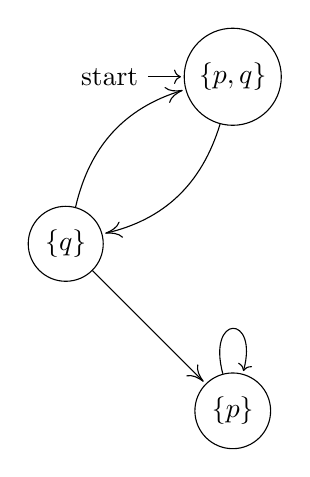
\begin{tikzpicture}[shorten >=1pt,node distance=3cm,on grid,auto] 
   	\node[state,initial](s_1){$\lbrace p,q\rbrace$}; 
   	\node[state](s_2)[below left=of s_1]{$\lbrace q\rbrace$};
   	\node[state](s_3)[below right=of s_2]{$\lbrace p\rbrace$};
    \path[-{>[scale=2,length=3,width=3]}] 
    (s_1) edge [bend left] node {} (s_2)
    (s_2) edge [bend left] node {} (s_1)
    	  edge node {} (s_3)
    (s_3) edge [loop above] node {} ();
\end{tikzpicture}
\caption{Ví dụ về cấu trúc Kripke}
\label{fig:KripkeStruct}
\end{figure}

\hspace{0.5cm}Với mô hình \ref {fig:KripkeStruct}, cho $AP = \lbrace p,q\rbrace$. Một cấu trúc Kripke $M = (S, S_0, R, L)$ được xác định với: $S = \lbrace s_1, s_2, s_3 \rbrace$, $S_0 = \lbrace s_1 \rbrace$, $R = \lbrace (s_1, s_2), (s_2, s_1), (s_2, s_3), (s_3, s_3)$ và $L = \lbrace (s_1,\lbrace p,q \rbrace), (s_2,\lbrace q \rbrace), (s_3,\lbrace p \rbrace) \rbrace$	 

\subsection{Logic có yếu tố thời gian}

\hspace{0.5cm}Logic yếu tố thời gian là mở rộng của logic mệnh đề truyền thống với việc kết hợp các toán tử mô tả được hành vi của hệ thống theo thời gian. Logic yếu tố thời gian cho phép mô tả được các tính chất của hệ thống thực như tính correctness, reachability, safety, liveness, fairness. Các toán tử được sự dụng để mô tả các hành vi của hệ thống theo thời gian là Path quantifiers và Temporal operators trong đó.

\begin{itemize}
\item{Path quantifiers: trong một biểu thức logic yếu tố thời gian được sử dụng để mô tả cấu trúc nhánh trong một cây tính toán. Trong đó 2 path quantifiers được sử dụng trong một biểu thức logic tính toán cây là $A$, mô tả với mọi đường tính toán, và $E$, mô tả tồn tại một đường tính toán.\\}
\item{Temporal operators: trong một biểu thức logic yếu tố thời gian được sử dụng để mô tả tính chất của một đường tính toán trong một cây tính toán. Trong đó 4 temporal operators được sử dụng trong một biểu thức tính toán cây là $X, F, G, U$.}
\end{itemize}

\hspace{0.5cm}\textbf{Toán tử $X$("neXt")}: $X\varphi$ mô tả trạng thái tiếp theo trên một đường tính toán thoả mãn tính chất $\varphi$.
\begin{figure}
\centering
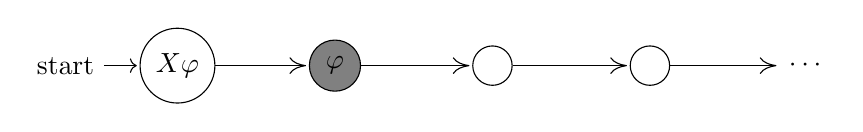
\begin{tikzpicture}[shorten >=1pt,node distance=2cm,on grid,auto] 
   	\node[state,initial,align=center,minimum size=0.5cm](s_0){$X\varphi$}; 
   	\node[state,align=center,minimum size=0.5cm,fill=gray](s_1)[right=of s_0]{$\varphi$};
   	\node[state,align=center,minimum size=0.5cm](s_2)[right=of s_1]{};
   	\node[state,align=center,minimum size=0.5cm](s_3)[right=of s_2]{};
   	\node (s_dots) [right=of s_3] {$\cdots$}; 
    \path[-{>[scale=2,length=3,width=3]}] 
    (s_0) edge node {} (s_1)
    (s_1) edge node {} (s_2)
    (s_2) edge node {} (s_3)
    (s_3) edge node {} (s_dots);
\end{tikzpicture}
\caption{Toán tử thời gian $X$}
\label{fig:NextTemporal}
\end{figure}

\hspace{0.5cm}\textbf{Toán tử $F$("Finally")}: $F\varphi$ mô tả một trạng thái bất kì trong tương lai thoả mãn tính chất $\varphi$.
\begin{figure}
\centering
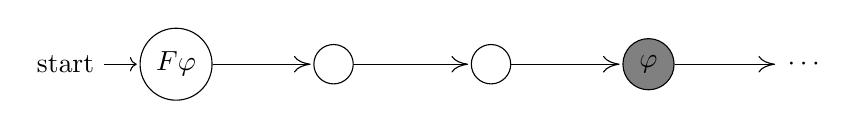
\begin{tikzpicture}[shorten >=1pt,node distance=2cm,on grid,auto] 
   	\node[state,initial,align=center,minimum size=0.5cm](s_0){$F\varphi$}; 
   	\node[state,align=center,minimum size=0.5cm](s_1)[right=of s_0]{};
   	\node[state,align=center,minimum size=0.5cm](s_2)[right=of s_1]{};
   	\node[state,align=center,minimum size=0.5cm,fill=gray](s_3)[right=of s_2]{$\varphi$};
   	\node (s_dots) [right=of s_3] {$\cdots$}; 
    \path[-{>[scale=2,length=3,width=3]}] 
    (s_0) edge node {} (s_1)
    (s_1) edge node {} (s_2)
    (s_2) edge node {} (s_3)
    (s_3) edge node {} (s_dots);
\end{tikzpicture}
\caption{Toán tử thời gian $F$}
\label{fig:FutureTemporal}
\end{figure}

\hspace{0.5cm}\textbf{Toán tử $G$("Globally")}: $G\varphi$ mô tả tất cả trạng thái trong tương lai thoả mãn tính chất $\varphi$.
\begin{figure}
\centering
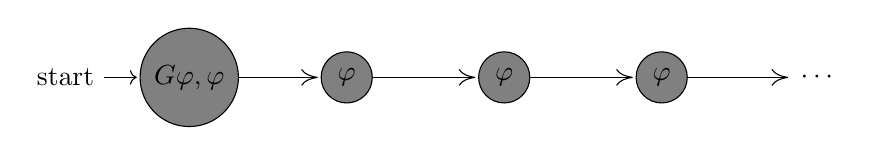
\begin{tikzpicture}[shorten >=1pt,node distance=2cm,on grid,auto] 
   	\node[state,initial,align=center,minimum size=0.5cm,fill=gray](s_0){$G\varphi,\varphi$}; 
   	\node[state,align=center,minimum size=0.5cm,fill=gray](s_1)[right=of s_0]{$\varphi$};
   	\node[state,align=center,minimum size=0.5cm,fill=gray](s_2)[right=of s_1]{$\varphi$};
   	\node[state,align=center,minimum size=0.5cm,fill=gray](s_3)[right=of s_2]{$\varphi$};
   	\node (s_dots) [right=of s_3] {$\cdots$}; 
    \path[-{>[scale=2,length=3,width=3]}] 
    (s_0) edge node {} (s_1)
    (s_1) edge node {} (s_2)
    (s_2) edge node {} (s_3)
    (s_3) edge node {} (s_dots);
\end{tikzpicture}
\caption{Toán tử thời gian $G$}
\label{fig:GlobalTemporal}
\end{figure}


\hspace{0.5cm}\textbf{Toán tử $U$("Until")}: $\varphi_1U\varphi_2$ mô tả tính chất $\varphi_1$ thoả mãn trên tất cả trạng thái cho đến khi tính chất $\varphi_2$ thoả mãn.
\begin{figure}
\centering
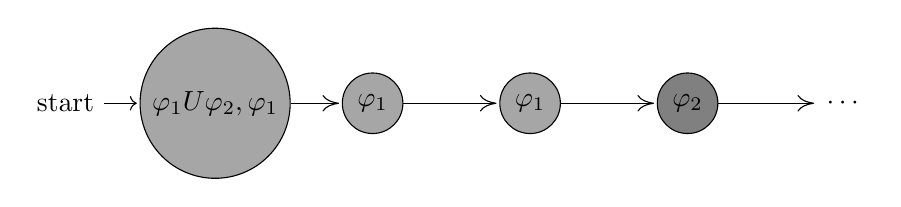
\begin{tikzpicture}[shorten >=1pt,node distance=2cm,on grid,auto] 
   	\node[state,initial,align=center,minimum size=0.5cm,fill=white!30!gray](s_0){$\varphi_1 U \varphi_2,\varphi_1$}; 
   	\node[state,align=center,minimum size=0.5cm,fill=white!30!gray](s_1)[right=of s_0]{$\varphi_1$};
   	\node[state,align=center,minimum size=0.5cm,fill=white!30!gray](s_2)[right=of s_1]{$\varphi_1$};
   	\node[state,align=center,minimum size=0.5cm,fill=gray](s_3)[right=of s_2]{$\varphi_2$};
   	\node (s_dots) [right=of s_3] {$\cdots$}; 
    \path[-{>[scale=2,length=3,width=3]}] 
    (s_0) edge node {} (s_1)
    (s_1) edge node {} (s_2)
    (s_2) edge node {} (s_3)
    (s_3) edge node {} (s_dots);
\end{tikzpicture}
\caption{Toán tử thời gian $U$}
\label{fig:UntilTemporal}
\end{figure}

\subsection{CTL}

\hspace{0.5cm}\textbf{Syntax}
\begin{code}
\begin{lstlisting}[captionpos=b,caption={CTL Syntax},label={lst:CTLSyntax},frame=single,mathescape=true]
$\Phi \Coloneqq true\;|\;p\;|\;(\neg\Phi)\;|\;(\Phi_1\wedge\Phi_2)\;|\;A\phi\;|\;E\phi$
$\phi \Coloneqq X\Phi\;|\;\Phi_1 U\Phi_2$
\end{lstlisting}
\end{code}

\hspace{0.5cm}\textbf{Semantic}
\begin{center}
\resizebox{10cm}{!}{
\begin{tikzpicture}[shorten >=1pt,node distance=1.5cm,on grid,auto] 
   	\node[state,initial,minimum size=0.5cm](s_1){}; 
   	\node[state, minimum size=0.5cm][below=of s_1](s_3){};
   	\node[state, minimum size=0.5cm][left=4cm of s_3](s_2){};
   	\node[state, minimum size=0.5cm][right=4cm of s_3,fill=red](s_4){};
   	\node[state, minimum size=0.5cm][below left=of s_2](s_5){};
   	\node[state, minimum size=0.5cm][below right=of s_2](s_6){};
   	\node[state, minimum size=0.5cm][below=1.06cm of s_3](s_7){};
   	\node[state, minimum size=0.5cm][below left=of s_4](s_8){};
	\node[state, minimum size=0.5cm][below right=of s_4](s_9){};
	\node[state, minimum size=0.5cm][below=1.2cm of s_5](s_10){};
	\node[state, minimum size=0.5cm][below left=1.7cm of s_7](s_11){};
	\node[state, minimum size=0.5cm][below right=1.7cm of s_7](s_12){};
	\node[state, minimum size=0.5cm][below=1.2cm of s_9](s_13){};
	\node[minimum size=0.5cm][below=of s_10](s_14){$\cdots$};
	\node[minimum size=0.5cm][below=of s_6](s_15){$\cdots$};
	\node[state, minimum size=0.5cm][below=of s_11](s_16){};
	\node[minimum size=0.5cm][below=of s_12](s_17){$\cdots$};
	\node[minimum size=0.5cm][below=of s_8](s_18){$\cdots$};
	\node[state,minimum size=0.5cm][below=of s_13](s_19){};
	\node[state,minimum size=0.5cm][below left=2.12cm of s_13](s_20){};
	\node[state,minimum size=0.5cm][below right=2.12cm of s_13](s_21){};
	\node[minimum size=0.5cm][below=of s_16](s_22){$\cdots$};
	\node[minimum size=0.5cm][below=of s_19](s_23){$\cdots$};
	\node[minimum size=0.5cm][below=of s_20](s_24){$\cdots$};
	\node[minimum size=0.5cm][below=of s_21](s_25){$\cdots$};
    \path[-{>[scale=2,length=3,width=3]}] 
    (s_1) edge node {} (s_2)
    	edge node {} (s_3)
    	edge node {} (s_4)
    (s_2) edge node {} (s_5)
    	edge node {} (s_6)
    (s_3) edge node {} (s_7)
    (s_4) edge node {} (s_8)
    	edge node {} (s_9)
    (s_5) edge node {} (s_10)
    (s_7) edge node {} (s_11)
    	edge node {} (s_12)
    (s_9) edge node {} (s_13)
    (s_11) edge node {} (s_16)
    (s_13) edge node {} (s_19)
    	edge node {} (s_20)
    	edge node {} (s_21);
\end{tikzpicture}
}\\
$M,s_0\models EX$\color{red}p
\end{center}

\begin{center}
\resizebox{10cm}{!}{
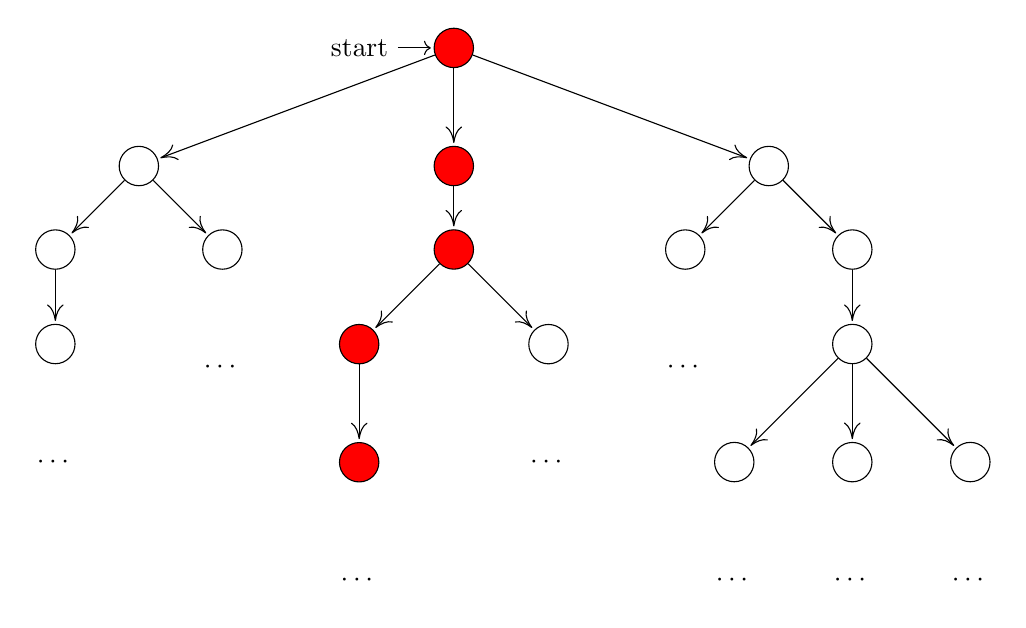
\begin{tikzpicture}[shorten >=1pt,node distance=1.5cm,on grid,auto] 
   	\node[state,initial,minimum size=0.5cm,fill=red](s_1){}; 
   	\node[state, minimum size=0.5cm][below=of s_1,fill=red](s_3){};
   	\node[state, minimum size=0.5cm][left=4cm of s_3](s_2){};
   	\node[state, minimum size=0.5cm][right=4cm of s_3](s_4){};
   	\node[state, minimum size=0.5cm][below left=of s_2](s_5){};
   	\node[state, minimum size=0.5cm][below right=of s_2](s_6){};
   	\node[state, minimum size=0.5cm][below=1.06cm of s_3,fill=red](s_7){};
   	\node[state, minimum size=0.5cm][below left=of s_4](s_8){};
	\node[state, minimum size=0.5cm][below right=of s_4](s_9){};
	\node[state, minimum size=0.5cm][below=1.2cm of s_5](s_10){};
	\node[state, minimum size=0.5cm][below left=1.7cm of s_7,fill=red](s_11){};
	\node[state, minimum size=0.5cm][below right=1.7cm of s_7](s_12){};
	\node[state, minimum size=0.5cm][below=1.2cm of s_9](s_13){};
	\node[minimum size=0.5cm][below=of s_10](s_14){$\cdots$};
	\node[minimum size=0.5cm][below=of s_6](s_15){$\cdots$};
	\node[state, minimum size=0.5cm][below=of s_11,fill=red](s_16){};
	\node[minimum size=0.5cm][below=of s_12](s_17){$\cdots$};
	\node[minimum size=0.5cm][below=of s_8](s_18){$\cdots$};
	\node[state,minimum size=0.5cm][below=of s_13](s_19){};
	\node[state,minimum size=0.5cm][below left=2.12cm of s_13](s_20){};
	\node[state,minimum size=0.5cm][below right=2.12cm of s_13](s_21){};
	\node[minimum size=0.5cm][below=of s_16](s_22){$\cdots$};
	\node[minimum size=0.5cm][below=of s_19](s_23){$\cdots$};
	\node[minimum size=0.5cm][below=of s_20](s_24){$\cdots$};
	\node[minimum size=0.5cm][below=of s_21](s_25){$\cdots$};
    \path[-{>[scale=2,length=3,width=3]}] 
    (s_1) edge node {} (s_2)
    	edge node {} (s_3)
    	edge node {} (s_4)
    (s_2) edge node {} (s_5)
    	edge node {} (s_6)
    (s_3) edge node {} (s_7)
    (s_4) edge node {} (s_8)
    	edge node {} (s_9)
    (s_5) edge node {} (s_10)
    (s_7) edge node {} (s_11)
    	edge node {} (s_12)
    (s_9) edge node {} (s_13)
    (s_11) edge node {} (s_16)
    (s_13) edge node {} (s_19)
    	edge node {} (s_20)
    	edge node {} (s_21);
\end{tikzpicture}
}\\
$M,s_0\models EG$\color{red}p
\end{center}

\begin{center}
\resizebox{10cm}{!}{
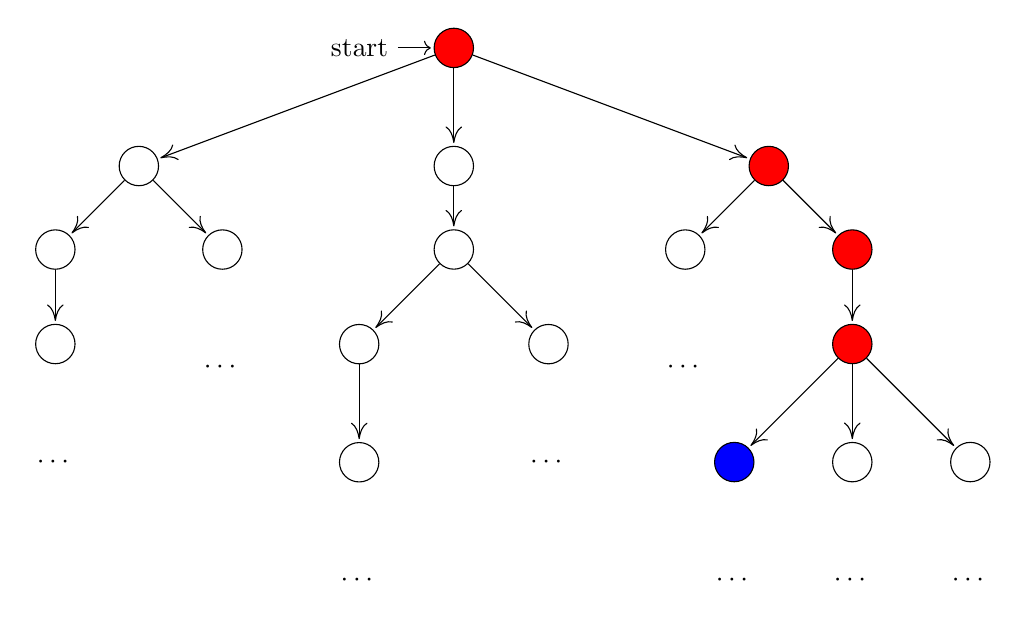
\begin{tikzpicture}[shorten >=1pt,node distance=1.5cm,on grid,auto] 
   	\node[state,initial,minimum size=0.5cm,fill=red](s_1){}; 
   	\node[state, minimum size=0.5cm][below=of s_1](s_3){};
   	\node[state, minimum size=0.5cm][left=4cm of s_3](s_2){};
   	\node[state, minimum size=0.5cm][right=4cm of s_3,fill=red](s_4){};
   	\node[state, minimum size=0.5cm][below left=of s_2](s_5){};
   	\node[state, minimum size=0.5cm][below right=of s_2](s_6){};
   	\node[state, minimum size=0.5cm][below=1.06cm of s_3](s_7){};
   	\node[state, minimum size=0.5cm][below left=of s_4](s_8){};
	\node[state, minimum size=0.5cm][below right=of s_4,fill=red](s_9){};
	\node[state, minimum size=0.5cm][below=1.2cm of s_5](s_10){};
	\node[state, minimum size=0.5cm][below left=1.7cm of s_7](s_11){};
	\node[state, minimum size=0.5cm][below right=1.7cm of s_7](s_12){};
	\node[state, minimum size=0.5cm][below=1.2cm of s_9,fill=red](s_13){};
	\node[minimum size=0.5cm][below=of s_10](s_14){$\cdots$};
	\node[minimum size=0.5cm][below=of s_6](s_15){$\cdots$};
	\node[state, minimum size=0.5cm][below=of s_11](s_16){};
	\node[minimum size=0.5cm][below=of s_12](s_17){$\cdots$};
	\node[minimum size=0.5cm][below=of s_8](s_18){$\cdots$};
	\node[state,minimum size=0.5cm][below=of s_13](s_19){};
	\node[state,minimum size=0.5cm][below left=2.12cm of s_13,fill=blue](s_20){};
	\node[state,minimum size=0.5cm][below right=2.12cm of s_13](s_21){};
	\node[minimum size=0.5cm][below=of s_16](s_22){$\cdots$};
	\node[minimum size=0.5cm][below=of s_19](s_23){$\cdots$};
	\node[minimum size=0.5cm][below=of s_20](s_24){$\cdots$};
	\node[minimum size=0.5cm][below=of s_21](s_25){$\cdots$};
    \path[-{>[scale=2,length=3,width=3]}] 
    (s_1) edge node {} (s_2)
    	edge node {} (s_3)
    	edge node {} (s_4)
    (s_2) edge node {} (s_5)
    	edge node {} (s_6)
    (s_3) edge node {} (s_7)
    (s_4) edge node {} (s_8)
    	edge node {} (s_9)
    (s_5) edge node {} (s_10)
    (s_7) edge node {} (s_11)
    	edge node {} (s_12)
    (s_9) edge node {} (s_13)
    (s_11) edge node {} (s_16)
    (s_13) edge node {} (s_19)
    	edge node {} (s_20)
    	edge node {} (s_21);
\end{tikzpicture}
}\\
$M,s_0\models E$\color{red}q$\;U\;$\color{blue}p
\end{center}

\begin{center}
\resizebox{10cm}{!}{
\begin{tikzpicture}[shorten >=1pt,node distance=1.5cm,on grid,auto] 
   	\node[state,initial,minimum size=0.5cm](s_1){}; 
   	\node[state, minimum size=0.5cm][below=of s_1](s_3){};
   	\node[state, minimum size=0.5cm][left=4cm of s_3](s_2){};
   	\node[state, minimum size=0.5cm][right=4cm of s_3](s_4){};
   	\node[state, minimum size=0.5cm][below left=of s_2](s_5){};
   	\node[state, minimum size=0.5cm][below right=of s_2,fill=red](s_6){};
   	\node[state, minimum size=0.5cm][below=1.06cm of s_3](s_7){};
   	\node[state, minimum size=0.5cm][below left=of s_4](s_8){};
	\node[state, minimum size=0.5cm][below right=of s_4](s_9){};
	\node[state, minimum size=0.5cm][below=1.2cm of s_5](s_10){};
	\node[state, minimum size=0.5cm][below left=1.7cm of s_7](s_11){};
	\node[state, minimum size=0.5cm][below right=1.7cm of s_7](s_12){};
	\node[state, minimum size=0.5cm][below=1.2cm of s_9](s_13){};
	\node[minimum size=0.5cm][below=of s_10](s_14){$\cdots$};
	\node[minimum size=0.5cm][below=of s_6](s_15){$\cdots$};
	\node[state, minimum size=0.5cm][below=of s_11](s_16){};
	\node[minimum size=0.5cm][below=of s_12](s_17){$\cdots$};
	\node[minimum size=0.5cm][below=of s_8](s_18){$\cdots$};
	\node[state,minimum size=0.5cm][below=of s_13](s_19){};
	\node[state,minimum size=0.5cm][below left=2.12cm of s_13](s_20){};
	\node[state,minimum size=0.5cm][below right=2.12cm of s_13](s_21){};
	\node[minimum size=0.5cm][below=of s_16](s_22){$\cdots$};
	\node[minimum size=0.5cm][below=of s_19](s_23){$\cdots$};
	\node[minimum size=0.5cm][below=of s_20](s_24){$\cdots$};
	\node[minimum size=0.5cm][below=of s_21](s_25){$\cdots$};
    \path[-{>[scale=2,length=3,width=3]}] 
    (s_1) edge node {} (s_2)
    	edge node {} (s_3)
    	edge node {} (s_4)
    (s_2) edge node {} (s_5)
    	edge node {} (s_6)
    (s_3) edge node {} (s_7)
    (s_4) edge node {} (s_8)
    	edge node {} (s_9)
    (s_5) edge node {} (s_10)
    (s_7) edge node {} (s_11)
    	edge node {} (s_12)
    (s_9) edge node {} (s_13)
    (s_11) edge node {} (s_16)
    (s_13) edge node {} (s_19)
    	edge node {} (s_20)
    	edge node {} (s_21);
\end{tikzpicture}
}\\
$M,s_0\models EF$\color{red}p
\end{center}

\begin{center}
\resizebox{10cm}{!}{
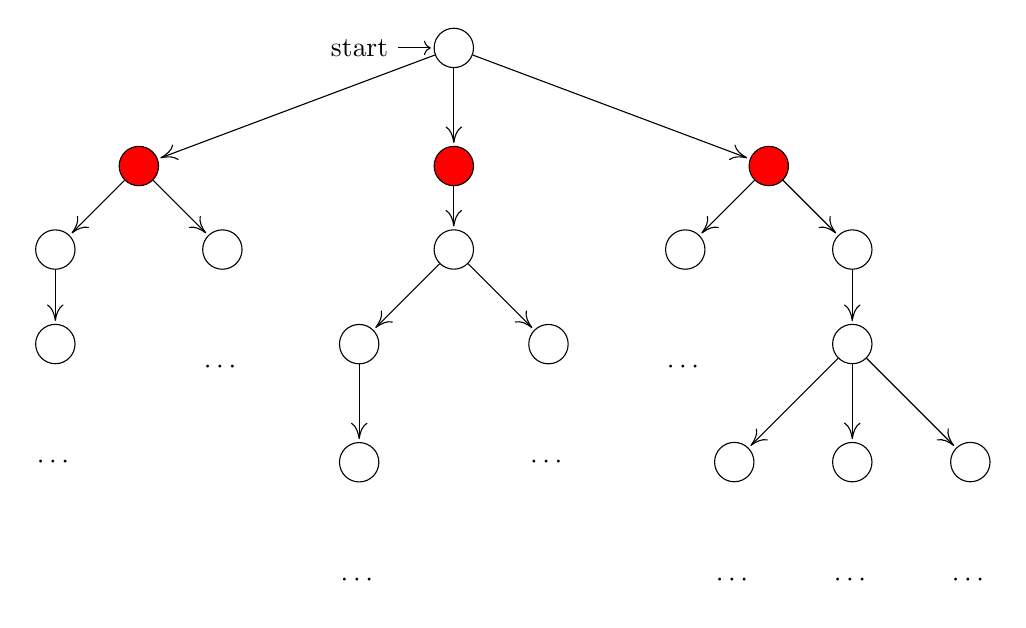
\begin{tikzpicture}[shorten >=1pt,node distance=1.5cm,on grid,auto] 
   	\node[state,initial,minimum size=0.5cm](s_1){}; 
   	\node[state, minimum size=0.5cm][below=of s_1,fill=red](s_3){};
   	\node[state, minimum size=0.5cm][left=4cm of s_3,fill=red](s_2){};
   	\node[state, minimum size=0.5cm][right=4cm of s_3,fill=red](s_4){};
   	\node[state, minimum size=0.5cm][below left=of s_2](s_5){};
   	\node[state, minimum size=0.5cm][below right=of s_2](s_6){};
   	\node[state, minimum size=0.5cm][below=1.06cm of s_3](s_7){};
   	\node[state, minimum size=0.5cm][below left=of s_4](s_8){};
	\node[state, minimum size=0.5cm][below right=of s_4](s_9){};
	\node[state, minimum size=0.5cm][below=1.2cm of s_5](s_10){};
	\node[state, minimum size=0.5cm][below left=1.7cm of s_7](s_11){};
	\node[state, minimum size=0.5cm][below right=1.7cm of s_7](s_12){};
	\node[state, minimum size=0.5cm][below=1.2cm of s_9](s_13){};
	\node[minimum size=0.5cm][below=of s_10](s_14){$\cdots$};
	\node[minimum size=0.5cm][below=of s_6](s_15){$\cdots$};
	\node[state, minimum size=0.5cm][below=of s_11](s_16){};
	\node[minimum size=0.5cm][below=of s_12](s_17){$\cdots$};
	\node[minimum size=0.5cm][below=of s_8](s_18){$\cdots$};
	\node[state,minimum size=0.5cm][below=of s_13](s_19){};
	\node[state,minimum size=0.5cm][below left=2.12cm of s_13](s_20){};
	\node[state,minimum size=0.5cm][below right=2.12cm of s_13](s_21){};
	\node[minimum size=0.5cm][below=of s_16](s_22){$\cdots$};
	\node[minimum size=0.5cm][below=of s_19](s_23){$\cdots$};
	\node[minimum size=0.5cm][below=of s_20](s_24){$\cdots$};
	\node[minimum size=0.5cm][below=of s_21](s_25){$\cdots$};
    \path[-{>[scale=2,length=3,width=3]}] 
    (s_1) edge node {} (s_2)
    	edge node {} (s_3)
    	edge node {} (s_4)
    (s_2) edge node {} (s_5)
    	edge node {} (s_6)
    (s_3) edge node {} (s_7)
    (s_4) edge node {} (s_8)
    	edge node {} (s_9)
    (s_5) edge node {} (s_10)
    (s_7) edge node {} (s_11)
    	edge node {} (s_12)
    (s_9) edge node {} (s_13)
    (s_11) edge node {} (s_16)
    (s_13) edge node {} (s_19)
    	edge node {} (s_20)
    	edge node {} (s_21);
\end{tikzpicture}
}\\
$M,s_0\models AX$\color{red}p
\end{center}

\begin{center}
\resizebox{10cm}{!}{
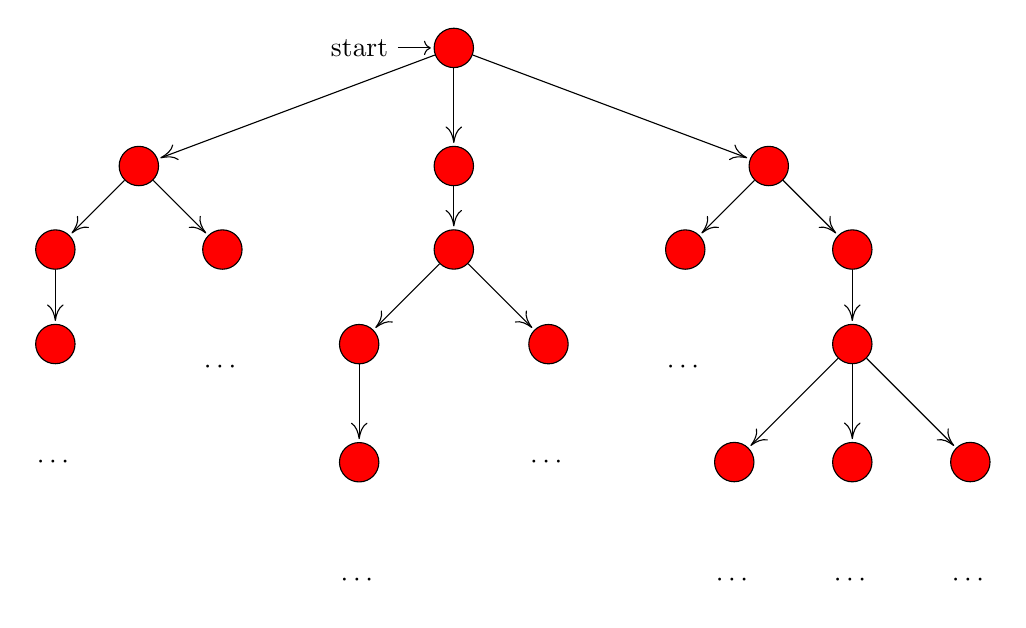
\begin{tikzpicture}[shorten >=1pt,node distance=1.5cm,on grid,auto] 
   	\node[state,initial,minimum size=0.5cm,fill=red](s_1){}; 
   	\node[state, minimum size=0.5cm][below=of s_1,fill=red](s_3){};
   	\node[state, minimum size=0.5cm][left=4cm of s_3,fill=red](s_2){};
   	\node[state, minimum size=0.5cm][right=4cm of s_3,fill=red](s_4){};
   	\node[state, minimum size=0.5cm][below left=of s_2,fill=red](s_5){};
   	\node[state, minimum size=0.5cm][below right=of s_2,fill=red](s_6){};
   	\node[state, minimum size=0.5cm][below=1.06cm of s_3,fill=red](s_7){};
   	\node[state, minimum size=0.5cm][below left=of s_4,fill=red](s_8){};
	\node[state, minimum size=0.5cm][below right=of s_4,fill=red](s_9){};
	\node[state, minimum size=0.5cm][below=1.2cm of s_5,fill=red](s_10){};
	\node[state, minimum size=0.5cm][below left=1.7cm of s_7,fill=red](s_11){};
	\node[state, minimum size=0.5cm][below right=1.7cm of s_7,fill=red](s_12){};
	\node[state, minimum size=0.5cm][below=1.2cm of s_9,fill=red](s_13){};
	\node[minimum size=0.5cm][below=of s_10](s_14){$\cdots$};
	\node[minimum size=0.5cm][below=of s_6](s_15){$\cdots$};
	\node[state, minimum size=0.5cm][below=of s_11,fill=red](s_16){};
	\node[minimum size=0.5cm][below=of s_12](s_17){$\cdots$};
	\node[minimum size=0.5cm][below=of s_8](s_18){$\cdots$};
	\node[state,minimum size=0.5cm][below=of s_13,fill=red](s_19){};
	\node[state,minimum size=0.5cm][below left=2.12cm of s_13,fill=red](s_20){};
	\node[state,minimum size=0.5cm][below right=2.12cm of s_13,fill=red](s_21){};
	\node[minimum size=0.5cm][below=of s_16](s_22){$\cdots$};
	\node[minimum size=0.5cm][below=of s_19](s_23){$\cdots$};
	\node[minimum size=0.5cm][below=of s_20](s_24){$\cdots$};
	\node[minimum size=0.5cm][below=of s_21](s_25){$\cdots$};
    \path[-{>[scale=2,length=3,width=3]}] 
    (s_1) edge node {} (s_2)
    	edge node {} (s_3)
    	edge node {} (s_4)
    (s_2) edge node {} (s_5)
    	edge node {} (s_6)
    (s_3) edge node {} (s_7)
    (s_4) edge node {} (s_8)
    	edge node {} (s_9)
    (s_5) edge node {} (s_10)
    (s_7) edge node {} (s_11)
    	edge node {} (s_12)
    (s_9) edge node {} (s_13)
    (s_11) edge node {} (s_16)
    (s_13) edge node {} (s_19)
    	edge node {} (s_20)
    	edge node {} (s_21);
\end{tikzpicture}
}\\
$M,s_0\models AG$\color{red}p
\end{center}

\begin{center}
\resizebox{10cm}{!}{
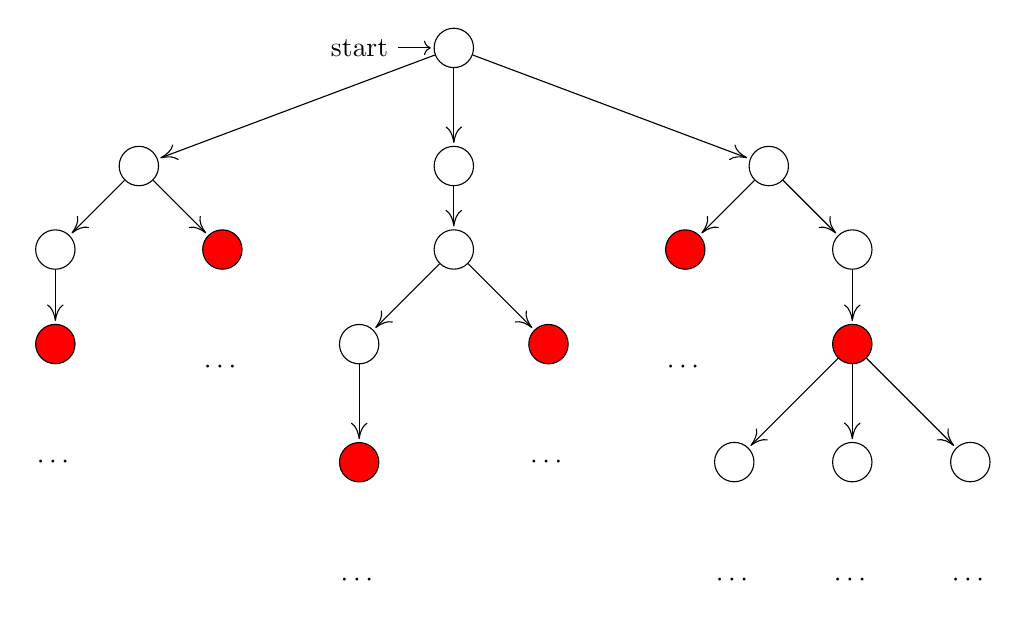
\begin{tikzpicture}[shorten >=1pt,node distance=1.5cm,on grid,auto] 
   	\node[state,initial,minimum size=0.5cm](s_1){}; 
   	\node[state, minimum size=0.5cm][below=of s_1](s_3){};
   	\node[state, minimum size=0.5cm][left=4cm of s_3](s_2){};
   	\node[state, minimum size=0.5cm][right=4cm of s_3](s_4){};
   	\node[state, minimum size=0.5cm][below left=of s_2](s_5){};
   	\node[state, minimum size=0.5cm][below right=of s_2,fill=red](s_6){};
   	\node[state, minimum size=0.5cm][below=1.06cm of s_3](s_7){};
   	\node[state, minimum size=0.5cm][below left=of s_4,fill=red](s_8){};
	\node[state, minimum size=0.5cm][below right=of s_4](s_9){};
	\node[state, minimum size=0.5cm][below=1.2cm of s_5,fill=red](s_10){};
	\node[state, minimum size=0.5cm][below left=1.7cm of s_7](s_11){};
	\node[state, minimum size=0.5cm][below right=1.7cm of s_7,fill=red](s_12){};
	\node[state, minimum size=0.5cm][below=1.2cm of s_9,fill=red](s_13){};
	\node[minimum size=0.5cm][below=of s_10](s_14){$\cdots$};
	\node[minimum size=0.5cm][below=of s_6](s_15){$\cdots$};
	\node[state, minimum size=0.5cm][below=of s_11,fill=red](s_16){};
	\node[minimum size=0.5cm][below=of s_12](s_17){$\cdots$};
	\node[minimum size=0.5cm][below=of s_8](s_18){$\cdots$};
	\node[state,minimum size=0.5cm][below=of s_13](s_19){};
	\node[state,minimum size=0.5cm][below left=2.12cm of s_13](s_20){};
	\node[state,minimum size=0.5cm][below right=2.12cm of s_13](s_21){};
	\node[minimum size=0.5cm][below=of s_16](s_22){$\cdots$};
	\node[minimum size=0.5cm][below=of s_19](s_23){$\cdots$};
	\node[minimum size=0.5cm][below=of s_20](s_24){$\cdots$};
	\node[minimum size=0.5cm][below=of s_21](s_25){$\cdots$};
    \path[-{>[scale=2,length=3,width=3]}] 
    (s_1) edge node {} (s_2)
    	edge node {} (s_3)
    	edge node {} (s_4)
    (s_2) edge node {} (s_5)
    	edge node {} (s_6)
    (s_3) edge node {} (s_7)
    (s_4) edge node {} (s_8)
    	edge node {} (s_9)
    (s_5) edge node {} (s_10)
    (s_7) edge node {} (s_11)
    	edge node {} (s_12)
    (s_9) edge node {} (s_13)
    (s_11) edge node {} (s_16)
    (s_13) edge node {} (s_19)
    	edge node {} (s_20)
    	edge node {} (s_21);
\end{tikzpicture}
}\\
$M,s_0\models AF$\color{red}p
\end{center}

\begin{center}
\resizebox{10cm}{!}{
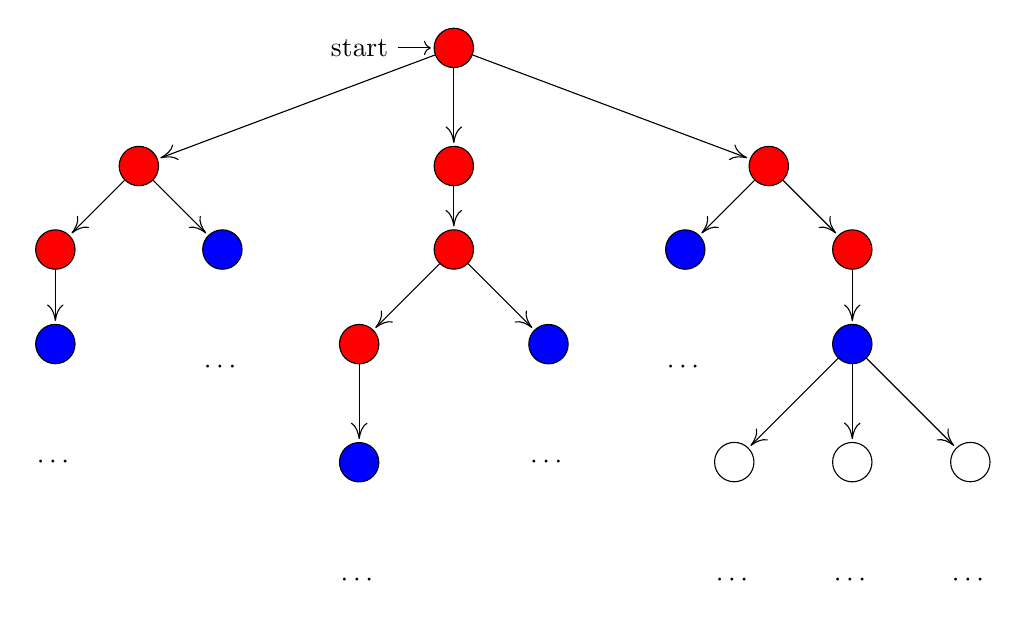
\begin{tikzpicture}[shorten >=1pt,node distance=1.5cm,on grid,auto] 
   	\node[state,initial,minimum size=0.5cm,fill=red](s_1){}; 
   	\node[state, minimum size=0.5cm][below=of s_1,fill=red](s_3){};
   	\node[state, minimum size=0.5cm][left=4cm of s_3,fill=red](s_2){};
   	\node[state, minimum size=0.5cm][right=4cm of s_3,fill=red](s_4){};
   	\node[state, minimum size=0.5cm][below left=of s_2,fill=red](s_5){};
   	\node[state, minimum size=0.5cm][below right=of s_2,fill=blue](s_6){};
   	\node[state, minimum size=0.5cm][below=1.06cm of s_3,fill=red](s_7){};
   	\node[state, minimum size=0.5cm][below left=of s_4,fill=blue](s_8){};
	\node[state, minimum size=0.5cm][below right=of s_4,fill=red](s_9){};
	\node[state, minimum size=0.5cm][below=1.2cm of s_5,fill=blue](s_10){};
	\node[state, minimum size=0.5cm][below left=1.7cm of s_7,fill=red](s_11){};
	\node[state, minimum size=0.5cm][below right=1.7cm of s_7,fill=blue](s_12){};
	\node[state, minimum size=0.5cm][below=1.2cm of s_9,fill=blue](s_13){};
	\node[minimum size=0.5cm][below=of s_10](s_14){$\cdots$};
	\node[minimum size=0.5cm][below=of s_6](s_15){$\cdots$};
	\node[state, minimum size=0.5cm][below=of s_11,fill=blue](s_16){};
	\node[minimum size=0.5cm][below=of s_12](s_17){$\cdots$};
	\node[minimum size=0.5cm][below=of s_8](s_18){$\cdots$};
	\node[state,minimum size=0.5cm][below=of s_13](s_19){};
	\node[state,minimum size=0.5cm][below left=2.12cm of s_13](s_20){};
	\node[state,minimum size=0.5cm][below right=2.12cm of s_13](s_21){};
	\node[minimum size=0.5cm][below=of s_16](s_22){$\cdots$};
	\node[minimum size=0.5cm][below=of s_19](s_23){$\cdots$};
	\node[minimum size=0.5cm][below=of s_20](s_24){$\cdots$};
	\node[minimum size=0.5cm][below=of s_21](s_25){$\cdots$};
    \path[-{>[scale=2,length=3,width=3]}] 
    (s_1) edge node {} (s_2)
    	edge node {} (s_3)
    	edge node {} (s_4)
    (s_2) edge node {} (s_5)
    	edge node {} (s_6)
    (s_3) edge node {} (s_7)
    (s_4) edge node {} (s_8)
    	edge node {} (s_9)
    (s_5) edge node {} (s_10)
    (s_7) edge node {} (s_11)
    	edge node {} (s_12)
    (s_9) edge node {} (s_13)
    (s_11) edge node {} (s_16)
    (s_13) edge node {} (s_19)
    	edge node {} (s_20)
    	edge node {} (s_21);
\end{tikzpicture}
}\\
$M,s_0\models A$\color{red}q$\;U\;$\color{blue}p
\end{center}

\subsection{Kiểm tra mô hình với NuSMV}

\hspace{0.5cm}Công cụ kiểm tra mô hình NuSMV được sử dụng để kiểm tra một mô hình có thoã mãn tính chất cần được kiểm tra hay không. Trong đó, mô hình cần kiểm tra sẽ được chuyển đổi qua mô hình NuSMV sử dụng ngôn ngữ SMV và tính chất cần được mô tả hình thức dưới dạng biểu thức logic CTL hoặc LTL.\\

\hspace{0.5cm}Ví dụ \ref {lst:NuSMVSample} sẽ trình bày cú pháp đơn giản để xây dựng một mô hình NuSMV, qua đó chuyển đổi một mô hình cơ bản quá trình thực thi của một tập tin tương ứng với mô hình \ref {lst:SampleExeASM} đã được trình bày ở trên, dưới dạng mô hình NuSMV. Cũng như sẽ mô tả một tính chất đơn giản để thực hiện việc kiểm tra trên mô hình này, giả sử tính chất cần được kiểm tra là: "Tồn tại một câu lệnh push một giá trị bất kì vào stack trong quá trình thực thi."

\begin{code}
\begin{lstlisting}[captionpos=b,caption={Ví dụ về kiểm tra mô hình trên NuSMV},label={lst:NuSMVSample},frame=single]
MODULE operand2(addr)
VAR
  op:{eax, undefined}
ASSIGN
  init(op):=undefined;
  next(op):=
    case
      (addr=0x00401000):eax;
      (addr=0x00401005):undefined;
      (addr=0x00401007):{eax, undefined};
      TRUE: undefined;
    esac;

MODULE operand1(addr)
VAR
  op:{0x00401007, eax, 0x00401005, ss:[esp], undefined}
ASSIGN
  init(op):=0x00401007;
  next(op):=
    case
      (addr=0x00401000):eax;
      (addr=0x00401005):0x00401005;
      (addr=0x00401007):{ss[esp], eax};
      TRUE: undefined;
    esac;

MODULE mnemonic(addr)
VAR
  mnem:{pushl, xorl, jne, movl, undefined}
ASSIGN
  init(mnem):=pushl;
  next(mnem):=
    case
      (addr=0x00401000):xor;
      (addr=0x00401005):jne;
      (addr=0x00401007):{call,xor};
      TRUE: undefined;
    esac;

MODULE state
VAR
  addr:{0x00401000,0x00401005,0x00401007,0x0040100B};
  mnem:mnemonic(addr);
  op1:operand1(addr);
  op2:operand2(addr);
ASSIGN
  init(addr):=0x00401000;
  next(addr):=
    case
      (addr=0x00401000):0x00401005;
      (addr=0x00401005):0x00401007;
      (addr=0x00401007):{0x0040100B,0x00401005};
      TRUE: addr;
    esac;

MODULE main
VAR
  s: state;

CTLSPEC AF(s.mnem == pushl)

\end{lstlisting}
\end{code}

\section{Các kỹ thuật chính của Packer}

\hspace{0.5cm}Hiện tại, hệ thống BE-PUM đã phân tích hoàn toàn được 27 packer. Các kỹ thuật trong 27 packer này được chia thành 6 nhóm bao gồm:

\begin{itemize}
\item{Code placing obfuscation: Dynamic Code và Code layout}
\item{Self-Modification: Dynamic Code, Code Overwriting, Overlapping Block}
\item{Instruction Obfuscation: Indirect Jump}
\item{Anti-tracing: Structured Exception Handler và 2 Special APIs}
\item{Arithmetic Operation: Obfuscated Constants và Checksumming}
\item{Anti-tampering: Checksumming, Anti-reversing, Anti-rewriting}
\end{itemize}

\subsection{Code placing obfuscation}\label{subsec:Packer1Tech}
\hspace{0.5cm}Nhóm kỹ thuật Code Placing Obfuscation bao gồm 2 nhóm kỹ thuật chính là: Dynamic Code và Code Layout.
\begin{enumerate}
\item{\textbf{Dynamic Code}: nhóm kỹ thuật Dynamic Code được sử dụng trong packer dưới dạng 2 kỹ thuật chính là Code Overwriting và kỹ thuật Packing/Unpacking.  
\begin{itemize}
\item{Kỹ thuật Code Overwriting: kỹ thuật này còn được gọi là kỹ thuật Self-modifying Code (SMC). Theo đó, packer sẽ sử dụng kỹ thuật này để có thể thay đổi động mã nhị phân của chương trình trong quá trình thực thi, chính vì giá trị này hay giá trị opcode thay đổi dẫn đến câu lệnh tại địa chỉ đó cũng được thay đổi. Packer sử dụng kỹ thuật này để có thể thay đổi chữ ký của mình vì thế đối với những phần mềm chống malware nhận dạng packer thông qua chữ ký sẽ không thể nhận dạng được vì chữ ký này luôn thay đổi liên tục. Chính vì hệ thống BE-PUM hỗ trợ giải thuật On-the-fly model generation với khả năng xử lý những thay động trong mã nhị phân mà hệ thống BE-PUM dễ dàng xử lý được kỹ thuật này. Đoạn mã \ref {lst:SMCinYODA} mô tả kỹ thuật Code Overwriting được sử dụng trong packer YODA. Theo đó sau khi thực thi đoạn mã tại vị trí 0x004040C6 với giá trị EDI = 0x004040C6, câu lệnh CMP đã được thay đổi thành câu lệnh MOV. 
\begin{code}
\begin{lstlisting}[captionpos=b,caption={Kỹ thuật Code Overwriting sử dụng trong packer YODA},label={lst:SMCinYODA},frame=single]
004040C3	stos es:[edi]
004040C6	cmp ecx, ebp

004040C3	stos es:[edi]
004040C6	mov ebp, ecx
\end{lstlisting}
\end{code}
}
\item{Kỹ thuật Packing/Unpacking: kỹ thuật này còn được gọi là kỹ thuật Encryption/Decryption, lõi của kỹ thuật này chính là kỹ thuật SMC đã được trình bày như trên, với số lượng vòng lặp được sử dụng để thay đổi một hoặc nhiều byte dẫn đến việc thay đổi câu lệnh liên tục trong suốt quá trình thực thi. Chính vì hệ thống BE-PUM có thể xử lý kỹ thuật SMC và hỗ trợ Dynamic symbolic execution mà giải thuật này dễ dàng được xử lý. Đoạn mã \ref {lst:PUinYODA} mô tả kỹ thuật packing/unpacking được sử dụng trong packer YODA.  
\begin{code}
\begin{lstlisting}[captionpos=b,caption={Kỹ thuật Packing/Unpacking sử dụng trong packer YODA},label={lst:PUinYODA},frame=single]
00404092	lods ds:[edi]
00404093	ror al, db
00404096	jmp 0x00404099
00404099	dec al
0040409B	add al,0x21
0040409D	dec al
0040409F	add al,cl
004040A1	stc
004040A2	add al,0x57
004040A4	clc
004040A5	add al,0x8A
004040A7	stc
004040A8	nop
004040A9	ror al,0xD7
004040AC	ror al,0x10
004040AF	jmp 0x004040B2
004040B2	ror al,0x5B
004040B5	clc
004040B6	xor al,0xD6
004040B8	stc
004040B9	xor al,0xD4
004040BB	sub al,cl
004040BD	jmp 0x004040C0 
004040C0	sub al,0x8B
004040C2	clc
004040C3	stos es:[edi]
004040C4	loopd 0x00404092
\end{lstlisting}
\end{code}
}
\end{itemize}
}
\item{\textbf{Code Layout}: nhóm kỹ thuật Code Layout được sử dụng trong packer dưới dạng 3 kỹ thuật chính là: Overlapping Functions, Overlapping Blocks và Code Chunking.
\begin{itemize}
\item{Kỹ thuật Overlapping Functions: kỹ thuật này với lõi là kỹ thuật Overlapping Instructions theo đó tại một địa chỉ bất kì trong phân cùng code mà có thể có rất nhiều câu lệnh mang giá trị tương ứng với các giá trị opcode khác nhau. Mỗi hàm được xác định với địa chỉ bắt đầu tại địa chỉ cũng là giá trị của toán hạng trong câu lệnh CALL và địa chỉ kết thúc chính là địa chỉ của câu lệnh RET trong cùng một hàm. Chính vì hệ thống BE-PUM hỗ trợ kỹ thuật On-the-fly nên kỹ thuật này cũng sẽ được BE-PUM xử lý không khó khăn.\\}
\item{Kỹ thuật Overlapping Blocks: kỹ thuật này cũng với lõi là kỹ thuật Overlapping Instructions. Khác với Overlapping Function mỗi khối được xác định và giới hạn thông qua câu lệnh nhảy hoặc nhảy có điều kiện. Đoạn mã \ref {lst:OBinYODA} mô tả kỹ thuật Overlapping Block được sử dụng trong packer YODA. Theo đó tại vị trí 0x004040BD một câu lệnh nhảy sẽ nhảy tới địa chỉ 0x004040C0 và tại địa chỉ này sẽ được dịch ngược thành một câu lệnh hoàn toàn khác. 
\begin{code}
\begin{lstlisting}[captionpos=b,caption={Kỹ thuật Overlapping Block sử dụng trong packer YODA},label={lst:OBinYODA},frame=single]
0040409D	dec al
0040409F	add al, cl
...
004040BF	retn 0x8B2C		
004040C2	clc
004040C3	stos es:[edi]
004040C4	loopd 0x00404092
00404092	lods ds:[edi]
...		
004040BD	jmp 0x004040C0
\end{lstlisting}
\end{code}
}
\item{Kỹ thuật Code Chunking: kỹ thuật này được packer sử dụng để có thể chia đoạn mã thực thi thành nhiều khối, mỗi khối là một tập với số lệnh câu lệnh xử lý rất ít hay nói cách khác mỗi khối có kích thước là dưới 20 bytes, mỗi khối này kết thúc với một câu lệnh nhảy. Hệ thống BE-PUM sử dụng kỹ thuật Dynamic symbolic execution để xử lý các câu lệnh nhảy do đó hệ thống BE-PUM cũng dễ dàng xử lý các kỹ thuật này. Đoạn mã \ref {lst:CCinYODA} mô tả kỹ thuật Code Chunking trong packer YODA, trong đó có thể thấy đoạn mã được chia nhỏ làm các khối 0x0040446E, 0x004474, 0x00404477, 0x0040447A.
\begin{code}
\begin{lstlisting}[captionpos=b,caption={Kỹ thuật Code Chunking sử dụng trong packer YODA},label={lst:CCinYODA},frame=single]
0040446B jmp 0x0040446E
... 
0040446E stc 
... 
00404474 jmp 0x00404477
...
00404477 jmp 0x0040447A
...
0040447A jmp 0x0040447D 
... 
0040447D nop
\end{lstlisting}
\end{code}
}
\end{itemize}
}
\end{enumerate}

\subsection{Self-Modifcation}
\hspace{0.5cm}Nhóm kỹ thuật Self-Modification bao gồm kỹ thuật Dynamic Code, Code Overwriting, Overlapping Block như đã được trình bày cụ thể trong chương \ref {subsec:Packer1Tech}, cũng như hướng xử lý những kỹ thuật này trên hệ thống BE-PUM.

\subsection{Instruction Obfuscation}
\hspace{0.5cm}Nhóm kỹ thuật Instruction Obfuscation hay còn gọi là kỹ thuật Indirect Jump, kỹ thuật được sử dụng rất nhiều trong hầu hết các packer. Theo đó, địa chỉ của câu lệnh nhảy, nhảy có điều kiện hay câu lệnh gọi hàm, và trả về của hàm được lưu trữ trong thanh ghi, bộ nhớ hay stack. Kỹ thuật Indirect Jump bao gồm 3 dạng: Indirect Call - giá trị đích được lưu trong lệnh gọi hàm CALL, Indirect Jump - giá trị đích được lưu trong lệnh nhảy hay nhảy có điều kiện, và Indirect Return - giá trị đích được xác định thông qua giá trị của thanh ghi ESP, do đó một packer sẽ thay đổi giá trị này và gọi lệnh trả về hàm để nhảy tới vị trí tại đỉnh của stack. Hệ thống BE-PUM sử dụng kỹ thuật Dynamic symbolic execution do đó hệ thống BE-PUM có thể dễ dàng xử lý được kỹ thuật này. Đoạn mã \ref {lst:IJinUPX} mô tả một ví dụ về việc sử dụng kỹ thuật Indirect Call trong packer UPX, theo đó giá trị đích nhảy đến được tính toán qua giá trị trong thanh ghi ESI.
\begin{code}
\begin{lstlisting}[captionpos=b,caption={Kỹ thuật Indirect Jump sử dụng trong packer UPX},label={lst:IJinUPX},frame=single]
004053FA  call ds:[esi+503C]
\end{lstlisting}
\end{code}

\subsection{Anti-tracing}
\hspace{0.5cm}Nhóm kỹ thuật Anti-tracing bao gồm 2 kỹ thuật chính là: Structured Exception Handler (SEH) và Two Special APIs.

\begin{itemize}
\item{Kỹ thuật SEH: bao gồm 2 giai đoạn chính. Trong giai đoạn đầu, packer sẽ thiết lập một ngoại lệ bằng cách sử dụng câu lệnh để có thể lưu trữ địa chỉ của hàm xử lý ngoại lệ trong thanh ghi FS:[0], giai đoạn này được gọi là Setup Exception. Khi một ngoại lệ xảy ra do thực hiện câu lệnh chia cho 0, đọc hoặc ghi vào vùng bộ nhớ không hợp lệ, hoặc khi Trap Flag được thiết lập giá trị FALSE, và khi packer cố tình sử dụng những câu lệnh ngắt như: INT3, INT68,...hệ thống khi đó sẽ tự động chuyển qua hàm xử lý ngoại lệ, giai đoạn này được gọi là Causing Exception. BE-PUM giải quyết vấn đề xử lý SEH bằng cách giả lập thanh ghi FS chứa giá trị địa chỉ của hàm xử lý ngoại lệ và lưu trữ danh sách các hàm xử lý ngoại lệ này. Ngoài ra, để kiểm tra ngoại lệ, BE-PUM kiểm tra câu lệnh là hợp lệ hay không, nếu không sẽ thực hiện chuyển đổi ngữ cảnh stack để thực hiện xử lý ngoại lệ, chính vì thế BE-PUM có thể dễ dàng xử lý được kỹ thuật này. Đoạn mã \ref {lst:SEHinPETITE} mô tả một ví dụ về việc sử dụng kỹ thuật SEH trong packer PETITE, theo đó có thể thấy 2 giai đoạn: Setup Exception tại vị trí 0x00404122 và Causing Exception tại vị trí 0x0040421E.
\begin{code}
\begin{lstlisting}[captionpos=b,caption={Kỹ thuật SEH sử dụng trong packer PETITE},label={lst:SEHinPETITE},frame=single]
00404116  push 0x004022E3
0040411B  push fs:[0]
00404122  mov fs:[0], esp
...
0040421E  mov ds:[edi],al
\end{lstlisting}
\end{code}
}
\item{Kỹ thuật Two Special APIs: trong kỹ thuật này, packer sẽ không nạp tất cả API cần sử dụng mà thay vào đó, packer sẽ chỉ nạp 2 API đặc biệt là: LoadLibrary và GetProcAddress để có thể lấy được địa chỉ của các API sẽ sử dụng. Hệ thống BE-PUM đã hỗ trợ 2 API đặc biệt này nên dễ dàng xử lý kỹ thuật.
\begin{code}
\begin{lstlisting}[captionpos=b,caption={Kỹ thuật Two Special APIs sử dụng trong packer FSG},label={lst:TwoAPIinFSG},frame=single]
004001C5  push eax
004001C6  call kernel32.LoadLibrary
...
004001D4  push eax
004001D5  push ebp
004001D6  call kernel32.GetProcAddress
\end{lstlisting}
\end{code}
}
\end{itemize}

\subsection{Arithmetic Operation}\label{subsec:Packer5Tech}
\hspace{0.5cm}Nhóm kỹ thuật Arithmetic Operation bao gồm 2 kỹ thuật chính bao gồm: Obfuscated Constants và Checksumming.

\begin{itemize}
\item{Kỹ thuật Obfuscated Constants: trong kỹ thuật này, thay vào việc sử dụng trực tiếp một gía trị hằng số, hay một số giá trị hexa cụ thể thì packer sẽ sử dụng rất nhiều câu lệnh tính toán phức tạp nhưng vẫn cho ra một hằng số mong muốn. Mục đích cụ thể là nâng cao độ phức tạp trong tính toán và làm rối rắm quá trình xử lý. Hệ thống BE-PUM hiện tại hỗ trợ hơn 200 câu lệnh hợp ngữ do đó việc tính toán các câu lệnh này là khả thi, tuy sẽ còn một số hạn chế nếu như packer sử dụng những câu lệnh tính toán mà hệ thống BE-PUM chưa hỗ trợ. Đoạn mã \ref {lst:OCinTELOCK} cho thấy quá trình sử dụng những câu lệnh XOR và SUB để tính toán một giá trị hằng số và được lưu trong thanh ghi EAX. 
\begin{code}
\begin{lstlisting}[captionpos=b,caption={Kỹ thuật Obfuscated Constants sử dụng trong packer TELOCK},label={lst:OCinTELOCK},frame=single]
00404C4B  mov eax, ss:[ebp + 40D280] 
00404C51  push eax
00404C52  xor eax, 7DCC805B 
00404C57  sub eax, 2A5DA2BD
\end{lstlisting}
\end{code}
}
\item{Kỹ thuật Checksumming: còn gọi là kỹ thuật CRC Checking, kỹ thuật này bao gồm 2 giai đoạn chính. Trong giai đoạn đầu, packer sẽ tính toán giá trị checksum với các giá trị xác định trong bộ nhớ, việc tính toán sẽ được tính toán qua các rất nhiều câu lệnh phức tạp cùng với số lần lặp là rất lớn. Trong giai đoạn tiếp theo, packer sẽ sử dụng một câu lệnh so sánh trực tiếp giá trị checksum này với một giá trị hằng số cụ thể để đảm bảo quá trình tính toán giá trị này cho ra một kết quả chính xác. Hệ thống BE-PUM hỗ trợ kỹ thuật Dynamic symbolic execution và phân tích trên giải thuật On-the-fly do đó hệ thống dễ dàng xử lý kỹ thuật này của packer. Đoạn mã \ref {lst:CSinTELOCK} biểu diễn hai quá trình của kỹ thuật Checksumming bao gồm việc tính toán giá trị checksum bắt đầu từ vị trí 0x004047F5 đến vị trí 00404806 và giai đoạn so sánh với giá trị hằng số 0x579122E6 tại vị trí 0x00404C57. 
\begin{code}
\begin{lstlisting} [captionpos=b,caption={Kỹ thuật Checksumming sử dụng trong packer TELOCK},label={lst:CSinTELOCK},frame=single]
004047F5  xor eax, eax
004047F7  lods ds:[edi]
004047F8  xor al, dl
004047FA  shr eax,0x1
00404806  inc ecx
00404812  jg 0x004047F5
...
00404C4B  mov eax, ss:[ebp + 40D280]
00404C51  push eax
00404C52  xor eax, 7DCC805B 
00404C57  sub eax, 2A5DA2BD
00404C63  jnz 0x0040527B
\end{lstlisting}
\end{code}
}
\end{itemize}

\subsection{Anti-tampering}
\hspace{0.5cm}Nhóm kỹ thuật Anti-tampering bao gồm các kỹ thuật chính: Anti-reversing, Anti-rewriting.

\begin{enumerate}
\item{\textbf{Anti-debugging}: Nhóm kỹ thuật Anti-debugging được sử dụng trong packer dưới dạng 3 kỹ thuật chính: Timming Check, Hardware Breakpoints, Anti-debugging.
\begin{itemize}
\item{Kỹ thuật Timing Check: trong kỹ thuật này, packer sẽ sử dụng những API có liên quan đến việc tính toán thời gian của hệ thống như: GetTickCount, GetSystemTime, GetLocalTime,...và những câu lệnh đặc biệt như RDTSC. Trong quá trình thực thi bình thường giá trị thời gian sẽ được tính toán bằng một hằng số cụ thể nhưng nếu tiến trình được xử lý trong môi trường debugger giá trị này sẽ được tính toán khác đi, do đó packer sẽ dễ dàng nhận dạng và kết thúc mở gói. Hệ thống BE-PUM đang dần mở rộng và hiện tại đã hỗ trợ hơn 400 API cũng như hỗ trợ nhiều hơn với các câu lệnh hợp ngữ do đó cũng sẽ xử lý được kỹ thuật này. Tuy nhiên sự tinh vi trong việc sử dụng này bằng cách sử dụng những API phức tạp hơn cũng chính là hạn chế mà hệ thống BE-PUM sẽ được mở rộng để hỗ trợ tốt hơn. Đoạn mã \ref {lst:TCinPECOMPACT} mô tả việc sử dụng API GetTickCount để lấy giá trị thời gian của hệ điều hành.
\begin{code}
\begin{lstlisting} [captionpos=b,caption={Kỹ thuật Timming Check sử dụng trong packer PECOMPACT},label={lst:TCinPECOMPACT},frame=single]
00404600  xor eax, eax
00404602  call GetTickCount
00404605  cmp eax, 0
00404608  jne 0x00404620
\end{lstlisting}
\end{code}
}
\item{Kỹ thuật Hardware Breakpoints: kỹ thuật này đã được trình bày như ví dụ cụ thể trong chương \ref {subsec:Example3}. Hệ thống BE-PUM được mở rộng để hỗ trợ thêm 8 thanh ghi debug do đó hệ thống BE-PUM cũng đã xử lý được kỹ thuật này.\\}
\item{Kỹ thuật Anti-debugging: trong kỹ thuật này, packer sẽ sử dụng những API để nhận dạng nếu tiến trình đang được thực thi trong môi trường debug như: IsDebuggerPresent, CheckRemoteDebuggerPresent, NtQueryInformationProcess,  NtQuerySystemInformation và NtQueryObject. Hệ thống BE-PUM cũng đã hỗ trợ các API nên việc xử lý kỹ thuật này là khả thi. 
\begin{code}
\begin{lstlisting}[captionpos=b,caption={Kỹ thuật Anti-debugging sử dụng trong packer YODA},label={lst:ADinYODA},frame=single]
00404888 call kernel32.IsDebuggerPresent
\end{lstlisting}
\end{code}
}
\end{itemize}
}
\item{\textbf{Anti-rewriting}: Nhóm kỹ thuật Anti-rewriting được sử dụng trong packer dưới dạng 2 kỹ thuật chính: Checksumming và Stolen Bytes trong đó kỹ thuật Checksumming đã được trình bày cụ thể ở chương \ref {subsec:Packer5Tech}.
\begin{itemize}
\item{Kỹ thuật Stolen Bytes: trong kỹ thuật này, packer sẽ cấp phát một vùng nhớ ảo đặc biệt bằng việc sử dụng API VirtualAlloc và ghi các byte giá trị bộ nhớ, cũng như mở gói trên vùng nhớ ảo này thay vì sử dụng kỹ thuật SMC. Kết thúc quá trình xử lý này, vùng nhớ ảo này sẽ ghi trở lại vào vùng nhớ thực và tiếp tục xử lý. Hệ thống BE-PUM đã hỗ trợ API VirtualAlloc và hiện thực vùng nhớ ảo cho bộ nhớ và các thao tác dịch ngược trên vùng nhớ ảo sử dụng Jackstab do đó hệ thống BE-PUM đã có thể xử lý kỹ thuật này.
\begin{code}
\begin{lstlisting}[captionpos=b,caption={Kỹ thuật Stolen Bytes sử dụng trong packer PECOMPACT},label={lst:SBinPECOMPACT},frame=single]
00404899  push edx
0040489A  mov ebp, eax
0040489C  push 0x40
0040489E  push 0x1000
004048A3  push ds:[ebx + 4]
004048A6  push 0
...   
004048AF  call kernel32.VirtualAlloc
\end{lstlisting}
\end{code}
}
\end{itemize}
}
\end{enumerate}



\section{Thiết kế giải thuật nhận dạng Packer thông qua chữ ký}

\section{Kết hợp hệ thống BE-PUM và NuSMV}

\subsection{Thiết kế và xây dựng NuSMV Model}

\subsection{Mô tả kỹ thuật Packer thông qua biểu thức CTL, LTL}

% ==========================================
% EXPERIMENTS AND RESULT
% ==========================================

\newpage
\chapter{THÍ NGHIỆM, ĐÁNH GIÁ VÀ KẾT LUẬN}

\section{Thí nghiệm và đánh giá kết quả}

\subsection{Kế hoạch thực hiện thí nghiệm}

\hspace{0.5cm}Công việc thực hiện thí nghiệm để có thể phân tích và nhận dạng packer được chia làm các bước sau:

\begin{itemize}
\item{Để có thể thí nghiệm phân tích packer trên hệ thống BE-PUM. Lựa chọn 9 tập tin mẫu và nén bằng 27 packer. Các tập tin mẫu bao gồm 5 tập tin tự tạo: api\_test.exe, demo1.exe, demo2.exe, bof.exe, api\_test\_v2.exe và 4 virus trong thực tế từ tập virus VXHeaven bao gồm: Virus.Win32.Aztec, Virus.Win32.Adson, Virus.Win32.Benny và Virus.Win32.Cabanas.2999.\\}
\item{Để có thể thí nghiệm nhận dạng packer qua kết hợp giữa hệ thống BE-PUM và công cụ NuSMV, lựa chọn từ tập virus LORIA 2000 virus và tiến hành chạy tự động.\\} 
\item{Để có thể đưa ra so sánh giữa hai phương pháp nhận dạng packer, một là thông qua phương pháp nhận dạng chữ ký và hai là phương pháp nhận dạng thông qua model checking. Thí nghiệm về nhận dạng packer thông qua chữ ký cũng sẽ được tiến hành.}
\end{itemize}

\hspace{0.5cm}Thí nghiệm được thực hiện trên hệ thống VMWare WinXP SP3, Intel Core i5 - 2450M 2.5GHz, 2GB RAM, JDK 1.8 và công cụ thực hiện kiểm tra mô hình NuSMV 2.6.0.

\subsection{Kết quả thí nghiệm}

\hspace{0.5cm}Kết quả thí nghiệm phân tích packer trên hệ thống BE-PUM được thể hiện trong bảng \ref {tab:27PackerExp}, bao gồm các 27 packer đã được hệ thống BE-PUM phân tích hoàn toàn, cũng như số node và edge được sinh ra sau khi phân tích các packer này.

\begin{small}
\setlength\tabcolsep{3pt}
\centering
\begin{longtable}{|l|l|l|l|}
\hline
\textbf{Tập tin nén api\_test.exe}	& \textbf{Nodes}	& \textbf{Edges}	& \textbf{Time}	\\
\hline 
ASPACK								& 1047				& 1112				& 58969 		\\
\hline 	
BJFNT								& 2061				& 2126				& 2810453		\\
\hline 
EXEPACK								& 323				& 353				& 6719			\\
\hline 
EXESTEALTH							& 735				& 770				& 238438		\\
\hline 
EXPRESSOR							& 1172				& 1233				& 76797			\\
\hline 
FSG									& 244				& 268				& 4000			\\
\hline 
LAME								& 235				& 244				& 10062			\\
\hline 
MEW									& 110				& 131				& 3187			\\
\hline 
MORPHNAH							& 228				& 232				& 3593			\\
\hline 
MPRESS								& 459				& 489				& 101391		\\
\hline 
NOODLECRYPT							& 706				& 757				& 33922			\\
\hline 
NPACK								& 602				& 639				& 9609			\\
\hline 
PECOMPACT							& 1127				& 1178				& 30891			\\
\hline 
PEECRYPT							& 511				& 517				& 26750			\\
\hline 
PETITE								& 1568				& 1635				& 49593			\\
\hline 
RLPACK								& 467				& 501				& 265937		\\
\hline 
SCRAMBLE v0.1						& 266				& 292				& 3984			\\
\hline 
SCRAMBLE v0.2						& 244				& 268				& 3922			\\
\hline 
TELOCK								& 2105				& 2237				& 6276360		\\
\hline 
UPACK								& 443				& 490				& 19625			\\
\hline 
UPX									& 323				& 353				& 6875			\\
\hline 
WINUPACK							& 443				& 490				& 19734			\\
\hline 
WWPACK32							& 329				& 360				& 3219			\\
\hline 
XCOMP								& 650				& 724				& 224734		\\
\hline 
YODA v1.2							& 625				& 659				& 130500		\\
\hline 
YODA v1.3							& 924				& 960				& 120516		\\
\hline 
PELOCK								& 2032				& 2033				& 36903693		\\
\hline 
PESPIN								& 431				& 452				& 4860547		\\
\hline
\caption {Kết quả thí nghiệm trên 27 packer}\label{tab:27PackerExp}
\end{longtable}
\end{small}

\hspace{0.5cm}Kết quả thí nghiệm nhận dạng 14 kỹ thuật trên 27 packer qua việc kết hợp giữa hệ thống BE-PUM và công cụ NuSMV được thể hiện trong bảng \ref {tab:27PackerSemanticExp}. \textit{Lưu ý:} Những ô kỹ thuật nào được đánh dấu "x" tương ứng với packer có sử dụng kỹ thuật đó.

\begin{tiny}
\setlength\tabcolsep{1pt}
\centering
\begin{longtable}{|l|c|c|c|c|c|c|c|c|c|c|c|c|c|c|}
\hline
\textbf{Packer}	& \textbf{\specialcell{Anti\\Debu\\gging}}	& \textbf{\specialcell{Check\\summ-\\ing}}	& \textbf{\specialcell{Code\\Chunk-\\ing}}		& \textbf{\specialcell{Indi-\\rect\\Jump}}		& \textbf{\specialcell{Obfus-\\cated\\Const-\\ants}}		& \textbf{\specialcell{Over-\\lapp-\\ing\\Block}}		& \textbf{\specialcell{Over-\\lapp-\\ing\\Func-\\tion}}		& \textbf{\specialcell{Over-\\writt-\\ing}}		& \textbf{\specialcell{Pack-\\ing\\Un-\\pack-\\ing}}	& \textbf{\specialcell{SEH}}	& \textbf{\specialcell{Stolen\\Bytes}}		& \textbf{\specialcell{Timm-\\ing\\Check}}		& \textbf{\specialcell{Two\\APIs}}		& \textbf{\specialcell{Hard-\\ware\\Break-\\points}} \\
\hline 
ASPACK				&	&x	&x	&x	&x	&x	&x	&x	&x	&	&x	&	&	&	\\
\hline
BJFNT				&	&x	&x	&	&x	&x	&	&x	&x	&	&	&	&	&	\\
\hline
EXEPACK				&	&x	&	&x	&x	&x	&	&x	&x	&	&	&	&x	&	\\
\hline
EXESTEALTH			&x	&x	&x	&x	&x	&x	&x	&x	&x	&x	&	&	&x	&	\\
\hline
EXPRESSOR			&	&x	&	&x	&x	&x	&x	&x	&x	&	&x	&	&	&	\\
\hline
FSG					&	&x	&	&x	&x	&x	&x	&x	&x	&	&	&	&x	&	\\
\hline
LAME				&	&x	&	&x	&x	&	&	&	&	&	&	&	&	&	\\
\hline
MEW					&	&x	&	&x	&x	&x	&x	&x	&x	&	&	&	&x	&	\\
\hline
MORPHNAH			&	&	&	&x	&x	&x	&	&	&	&	&	&	&	&	\\
\hline
MPRESS				&	&x	&	&x	&x	&x	&	&x	&x	&	&	&	&	&	\\
\hline
NOODLECRYPT			&	&x	&x	&x	&x	&x	&x	&	&	&	&	&	&x	&	\\
\hline
NPACK				&	&x	&	&x	&x	&x	&x	&x	&x	&	&x	&	&x	&	\\
\hline
PECOMPACT			&	&x	&	&x	&x	&x	&x	&x	&x	&x	&x	&	&x	&	\\
\hline
PEENCRYPT			&	&	&x	&x	&x	&x	&	&x	&x	&	&	&	&	&	\\
\hline
PETITE				&	&x	&	&x	&x	&x	&x	&x	&x	&x	&	&	&	&	\\
\hline
RLPACK				&	&x	&	&x	&x	&x	&x	&x	&x	&	&x	&	&x	&	\\
\hline
SCRAMBLE v0.1		&	&x	&	&x	&x	&x	&x	&x	&x	&	&	&	&x	&	\\
\hline
SCRAMBLE v0.2		&	&x	&	&x	&x	&x	&x	&x	&x	&	&	&	&x	&	\\
\hline
TELOCK				&	&x	&x	&x	&x	&x	&x	&x	&x	&x	&x	&	&	&x	\\
\hline
UPACK				&	&x	&	&x	&x	&x	&x	&x	&x	&	&	&	&x	&	\\
\hline
UPX					&	&x	&	&x	&x	&x	&	&x	&x	&	&	&	&x	&	\\
\hline
WINUPACK			&	&x	&	&x	&x	&x	&x	&x	&x	&	&	&	&x	&	\\
\hline
WWPACK32			&	&x	&	&	&x	&x	&x	&x	&x	&	&	&	&	&	\\
\hline
XCOMP				&	&x	&	&x	&x	&x	&x	&x	&x	&	&x	&	&x	&	\\
\hline
YODA v1.2			&x	&x	&	&x	&x	&x	&x	&x	&x	&x	&	&	&x	&	\\
\hline
YODA v1.3			&x	&x	&x	&x	&x	&x	&x	&x	&x	&x	&	&	&x	&	\\
\hline
PELOCK				&	&	&x	&	&x	&x	&	&x	&x	&	&	&	&	&	\\
\hline
PESPIN				&	&x	&x	&x	&x	&x	&x	&x	&x	&	&	&	&	&	\\			
\hline
\caption {Kết quả thí nghiệm nhận dạng trên 27 packer}\label{tab:27PackerSemanticExp}
\end{longtable}
\end{tiny}

\hspace{0.5cm}Với kết quả thí nghiệm trên 2000 virus từ tập virus LORIA, hình \ref {fig:PackerStat} thống kê số lượng từng packer được nhận dạng.

\begin{figure}
\centering
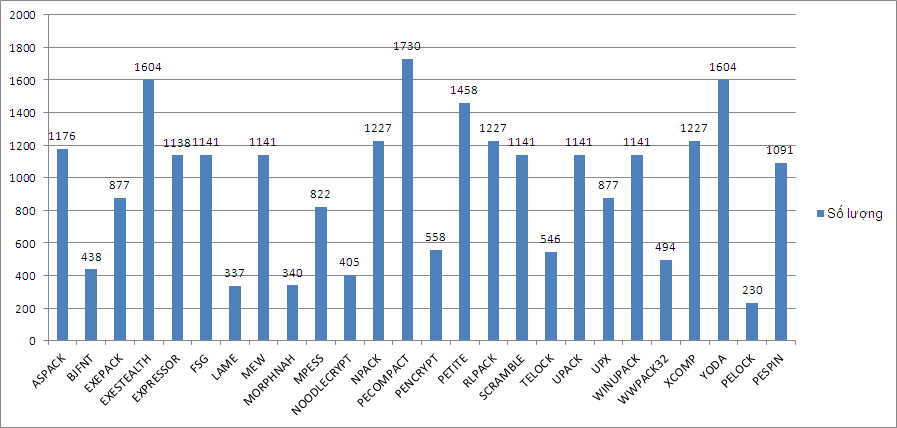
\includegraphics[width=0.8\textwidth]{packer_statistic}
\caption{Thống kê quá trình nhận dạng packer trên tập LORIA}
\label{fig:PackerStat}
\end{figure}

\hspace{0.5cm}Với kết quả thí nghiệm trên 2000 virus từ tập virus LORIA, hình \ref {fig:TechStat} thống kê số lượng từng kỹ thuật được packer sử dụng.

\begin{figure}
\centering
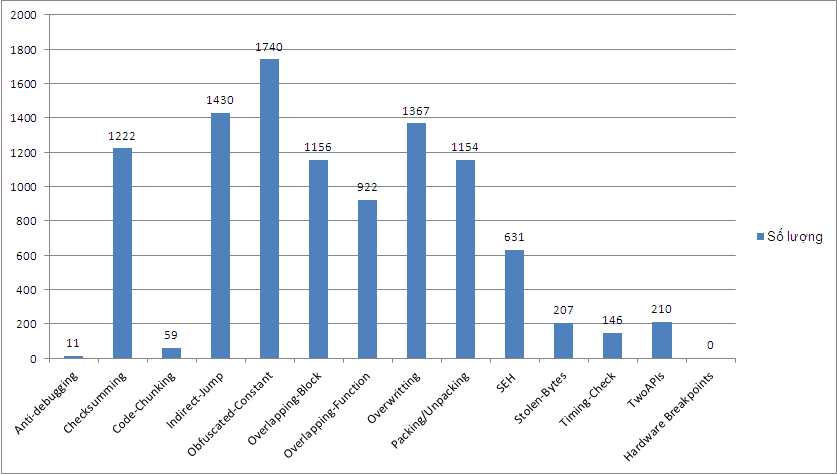
\includegraphics[width=0.8\textwidth]{technique_statistic}
\caption{Thống kê số lượng từng kỹ thuật của packer.}
\label{fig:TechStat}
\end{figure}

\section{Kết luận}

\hspace{0.5cm}Theo thống kê, số lượng những tập tin có kết quả nhận dạng packer thông qua chữ ký và thông qua ngữ nghĩa giống nhau là 335 trên tổng số 1942 malware được thí nghiệm. Điều này chứng tỏ quá trình nhận dạng thông qua ngữ nghĩa được thực hiện trong đề tài luận văn này còn những hạn chế nhất định và sẽ được cải tiến trong tương lai.\\

\hspace{0.5cm}Từ hình \ref {fig:TechStat} có thể thấy những kỹ thuật được sử dụng nhiều nhất trong packer là: Obfuscated Constants, Indirect Jump, Packing/Unpacking, Overwriting và Checksumming. Điều đó kết luận được rằng đó cũng là những kỹ thuật chính yếu được sử dụng trong packer, và tương lai sẽ tập trung cải thiện phân tích chính xác hơn các kỹ thuật này.



% ==========================================
% FUTURE WORKS
% ==========================================

\newpage
\chapter{HƯỚNG PHÁT TRIỂN TRONG TƯƠNG LAI}

\section{Hạn chế của đề tài}

\section{Mục tiêu hướng tới trong tương lai}



% ==========================================
% APPENDIX
% ==========================================

\newpage
\chapter{PHỤ LỤC}

\begin{thebibliography}{}

\end{thebibliography}

\end{document}



